\begin{componente}{CLIPS}
\compDescrizione{package generale contenente il prodotto del progetto}
\begin{compPackageContenuti}
\item CLIPS::client: componente globale per il front end del prodotto che utilizza il design pattern \gl{MVC}. Si occupa di fornire un'interfaccia grafica dell'applicazione e di interagire con il lato server.
\item CLIPS::server: componente globale per il back end del prodotto
\end{compPackageContenuti}
\end{componente}
\begin{componente}{CLIPS::client}
\begin{figure}[h!] 
\centering 
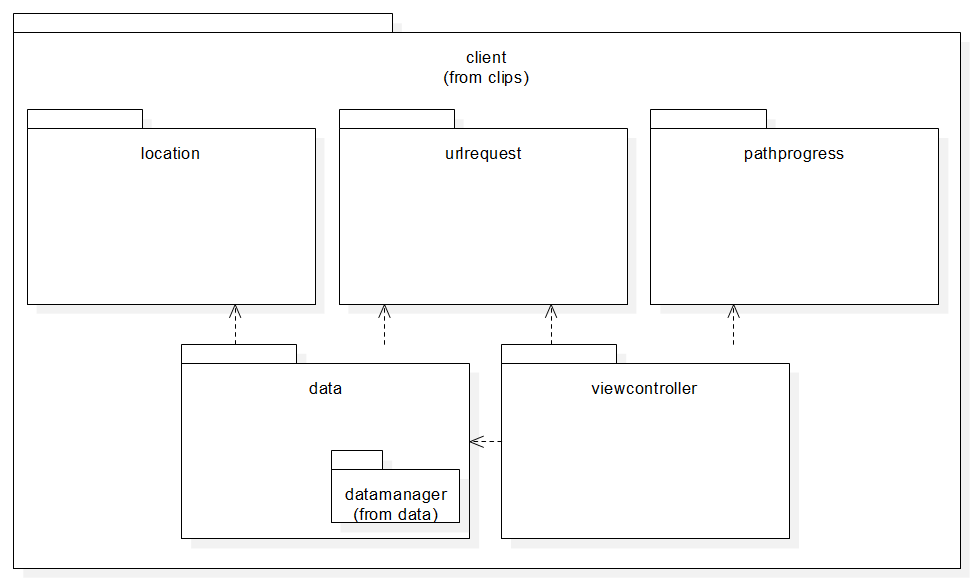
\includegraphics[scale=0.4]{img/package/png/client.png} 
\caption{Schema package client} 
 \end{figure} 
\compDescrizione{componente globale per il front end del prodotto che utilizza il design pattern \gl{MVC}. Si occupa di fornire un'interfaccia grafica dell'applicazione e di interagire con il lato server.}
\compPadre{CLIPS}
\begin{compPackageContenuti}
\item CLIPS::client::authentication: componente che si occupa di gestire l'autenticazione dell'utente
\item CLIPS::client::data: package per la gestione in locale dei dati
\item CLIPS::client::location: componente che gestisce l'individuazione e la lettura dei beacon
\item CLIPS::client::pathprogress: componente che gestisce i dati del percorso e salva i risultati ottenuti nelle prove mentre si sta giocando
\item CLIPS::client::viewcontroller: componente che raggruppa tutte le view ed i controller relativi alle view
\end{compPackageContenuti}
\end{componente}
\begin{componente}{CLIPS::client::authentication}
\begin{figure}[h!] 
\centering 
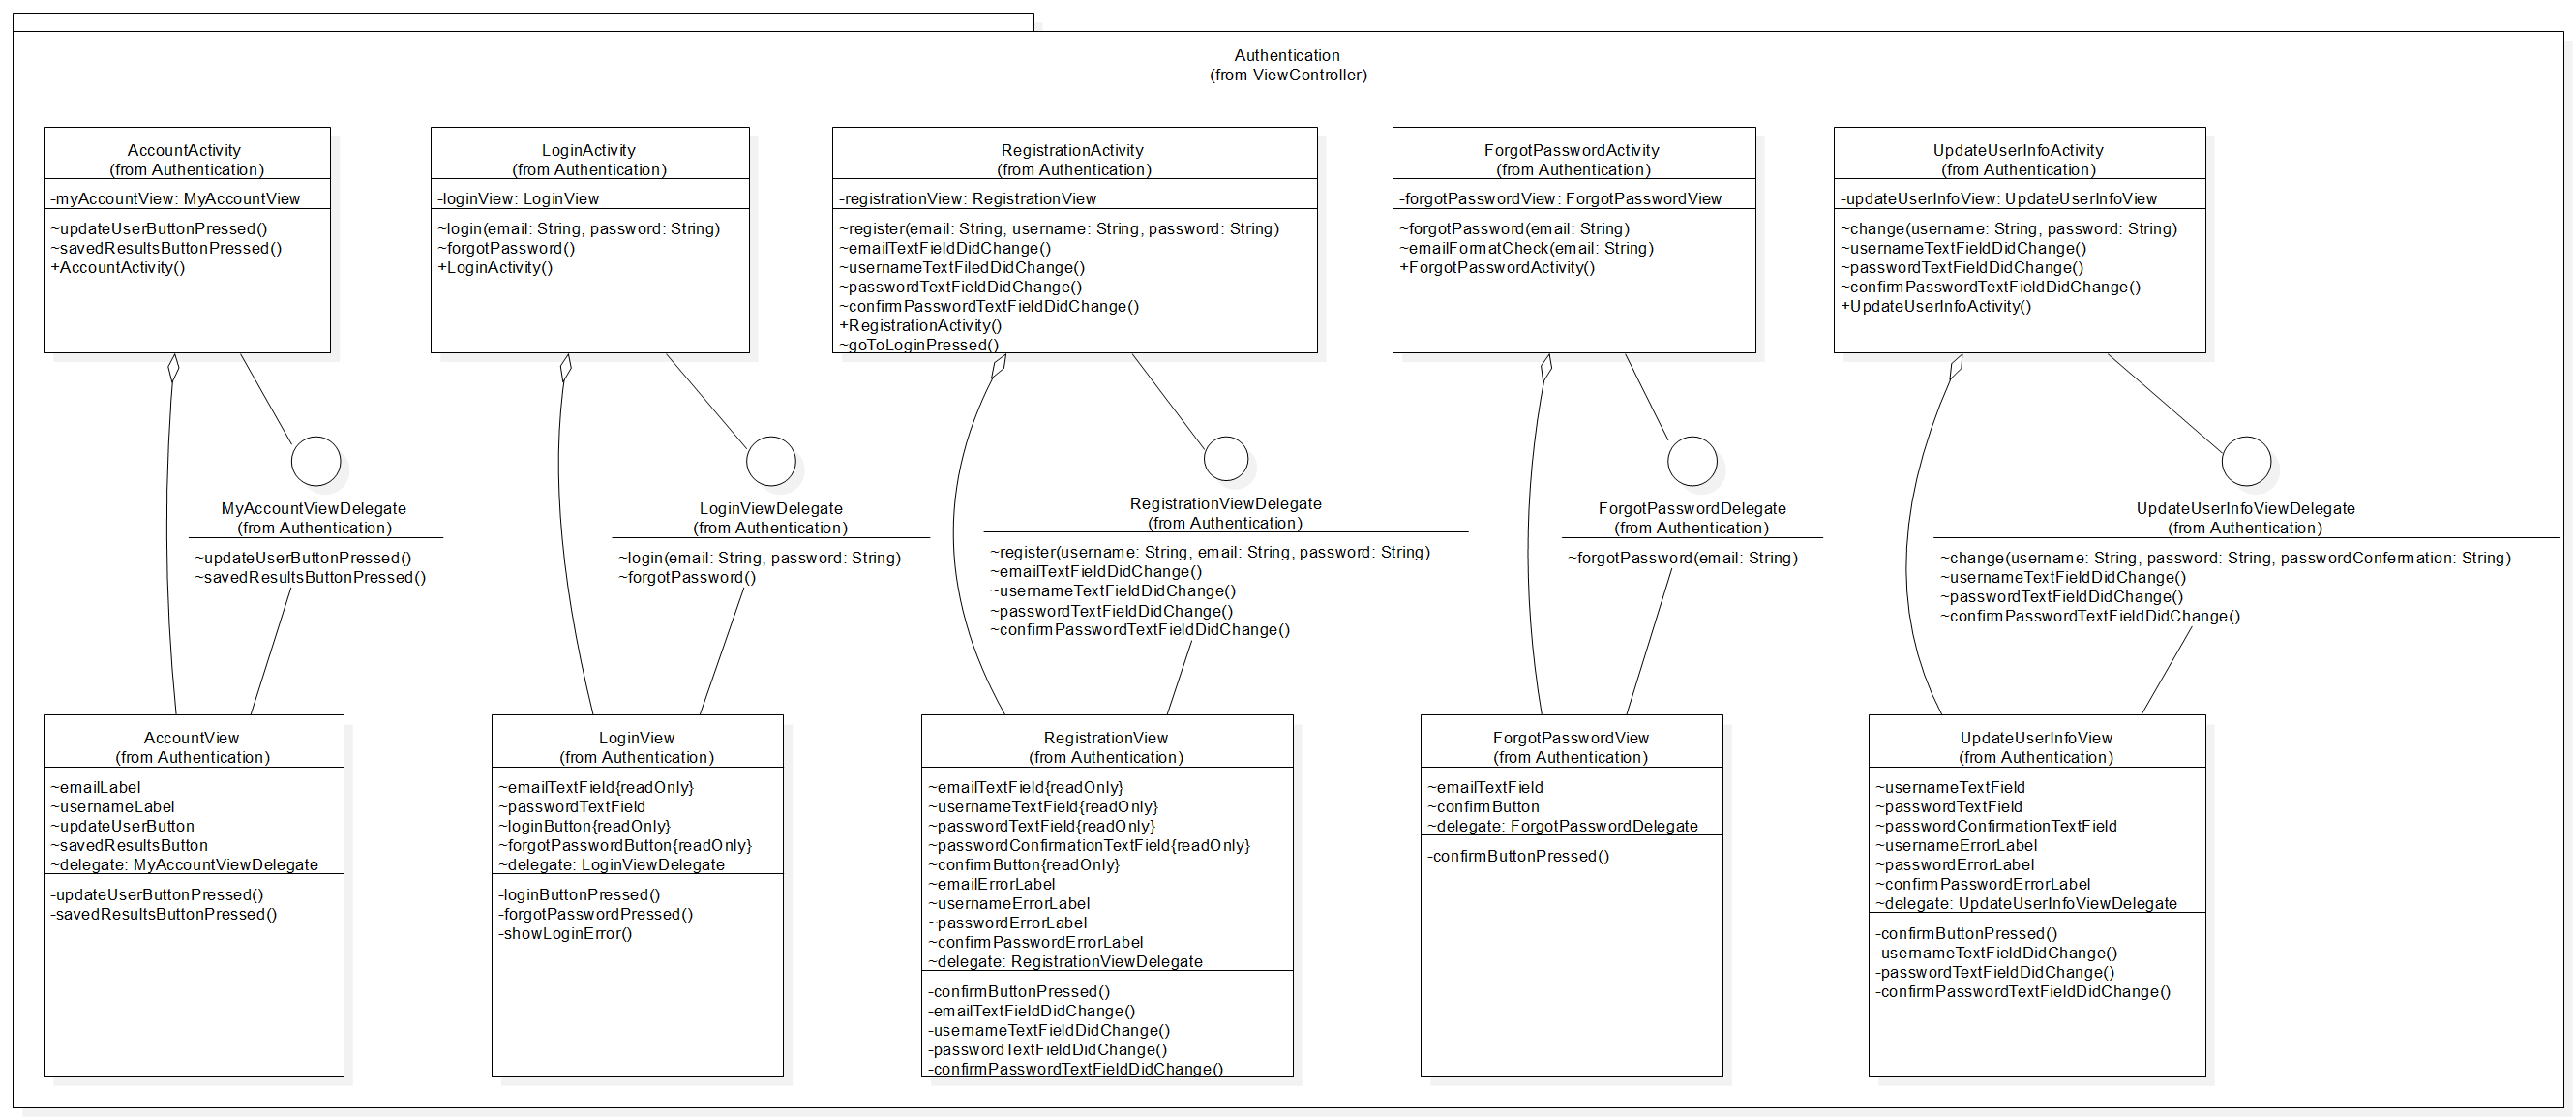
\includegraphics[scale=0.4]{img/package/png/client--viewcontroller--authentication.png} 
\caption{Schema package client::viewcontroller::authentication} 
 \end{figure} 
\compDescrizione{componente che si occupa di gestire l'autenticazione dell'utente}
\compPadre{client}
\begin{compClassi} \\ 
\begin{classe}{CLIPS::client::authentication::AccountActivity}
\classeDescrizione{classe controller che si occupa di interagire con AccountView}
\classeUtilizzo{si occupa di gestire le interazioni dell'utente con AccountView}
\begin{classeRelazioni}
\classeRelazione{CLIPS::client::authentication}{AccountViewDelegate}{interfaccia per segnalare gli eventi della classe AccountView}\end{classeRelazioni}
\end{classe}\begin{classe}{CLIPS::client::authentication::AccountView}
\classeDescrizione{classe che rappresenta la schermata delle informazioni dell'utente}
\classeUtilizzo{permette all'utente di visualizzare le informazioni del proprio profilo}
\begin{classeRelazioni}
\classeRelazione{CLIPS::client::authentication}{AccountActivity}{classe controller che si occupa di interagire con AccountView}\classeRelazione{CLIPS::client::authentication}{AccountViewDelegate}{interfaccia per segnalare gli eventi della classe AccountView}\end{classeRelazioni}
\end{classe}\begin{classe}{CLIPS::client::authentication::AccountViewDelegate}
\classeDescrizione{interfaccia per segnalare gli eventi della classe AccountView}
\classeUtilizzo{si occupa di fornire i metodi necessari alla classe AccountView per notificare gli eventi}
\begin{classeRelazioni}
\classeRelazione{CLIPS::client::authentication}{AccountActivity}{classe controller che si occupa di interagire con AccountView}\classeRelazione{CLIPS::client::authentication}{AccountView}{classe che rappresenta la schermata delle informazioni dell'utente}\end{classeRelazioni}
\end{classe}\begin{classe}{CLIPS::client::authentication::ForgotPasswordActivity}
\classeDescrizione{classe controller che si occupa di interagire con ForgotPasswordView}
\classeUtilizzo{si occupa di gestire le interazioni dell'utente con ForgotPasswordView}
\begin{classeRelazioni}
\classeRelazione{CLIPS::client::authentication}{ForgotPasswordView}{classe che si occupa della visualizzazione della schermata per la richiesta di una nuova password}\classeRelazione{CLIPS::client::authentication}{ForgotPasswordViewDelegate}{interfaccia per segnalare gli eventi della classe ForgotPasswordView}\end{classeRelazioni}
\end{classe}\begin{classe}{CLIPS::client::authentication::ForgotPasswordView}
\classeDescrizione{classe che si occupa della visualizzazione della schermata per la richiesta di una nuova password}
\classeUtilizzo{consente all'utente di inserire la mail per ricevere una nuova password}
\begin{classeAttributi}
\classeAttributo{emailTextField}{TextField}{text field dell'email}
\end{classeAttributi}
\begin{classeRelazioni}
\classeRelazione{CLIPS::client::authentication}{ForgotPasswordViewDelegate}{interfaccia per segnalare gli eventi della classe ForgotPasswordView}\end{classeRelazioni}
\end{classe}\begin{classe}{CLIPS::client::authentication::ForgotPasswordViewDelegate}
\classeDescrizione{interfaccia per segnalare gli eventi della classe ForgotPasswordView}
\classeUtilizzo{si occupa di fornire i metodi necessari alla classe ForgotPasswordView per notificare gli eventi}
\begin{classeRelazioni}
\classeRelazione{CLIPS::client::authentication}{ForgotPasswordActivity}{classe controller che si occupa di interagire con ForgotPasswordView}\classeRelazione{CLIPS::client::authentication}{ForgotPasswordView}{classe che si occupa della visualizzazione della schermata per la richiesta di una nuova password}\end{classeRelazioni}
\end{classe}\begin{classe}{CLIPS::client::authentication::LoginActivity}
\classeDescrizione{classe controller che si occupa di interagire con LoginView}
\classeUtilizzo{si occupa di gestire le interazioni dell'utente con LoginView}
\begin{classeRelazioni}
\classeRelazione{CLIPS::client::authentication}{LoginView}{classe che si occupa della visualizzazione della schermata per il login}\classeRelazione{CLIPS::client::authentication}{LoginViewDelegate}{interfaccia per segnalare gli eventi della classe LoginView}\end{classeRelazioni}
\end{classe}\begin{classe}{CLIPS::client::authentication::LoginView}
\classeDescrizione{classe che si occupa della visualizzazione della schermata per il login}
\classeUtilizzo{consente all'utente di inserire i propri dati per effettuare il login}
\begin{classeAttributi}
\classeAttributo{emailTextField}{string}{rappresenta l'email}
\end{classeAttributi}
\begin{classeMetodi}
\classeMetodo{forgotPasswordPressed()}{}{void}{invia un evento il quale notifica che il bottone di password dimenticata è stato premuto}
\classeMetodo{loginButtonPressed()}{}{void}{invia un evento di bottone del login premuto}
\end{classeMetodi}
\begin{classeRelazioni}
\classeRelazione{CLIPS::client::authentication}{LoginViewDelegate}{interfaccia per segnalare gli eventi della classe LoginView}\end{classeRelazioni}
\end{classe}\begin{classe}{CLIPS::client::authentication::LoginViewDelegate}
\classeDescrizione{interfaccia per segnalare gli eventi della classe LoginView}
\classeUtilizzo{si occupa di fornire i metodi necessari alla classe LoginView per notificare gli eventi}
\begin{classeRelazioni}
\classeRelazione{CLIPS::client::authentication}{LoginActivity}{classe controller che si occupa di interagire con LoginView}\classeRelazione{CLIPS::client::authentication}{LoginView}{classe che si occupa della visualizzazione della schermata per il login}\end{classeRelazioni}
\end{classe}\begin{classe}{CLIPS::client::authentication::RegistrationActivity}
\classeDescrizione{classe controller che si occupa di interagire con RegistrationView}
\classeUtilizzo{si occupa di gestire le interazioni dell'utente con RegistrationView}
\begin{classeRelazioni}
\classeRelazione{CLIPS::client::authentication}{RegistrationView}{classe che si occupa della visualizzazione della schermata per la registrazione}\classeRelazione{CLIPS::client::authentication}{RegistrationViewDelegate}{interfaccia per segnalare gli eventi della classe RegistrationView}\end{classeRelazioni}
\end{classe}\begin{classe}{CLIPS::client::authentication::RegistrationView}
\classeDescrizione{classe che si occupa della visualizzazione della schermata per la registrazione}
\classeUtilizzo{consente all'utente di inserire i propri dati per effettuare la registrazione}
\begin{classeRelazioni}
\classeRelazione{CLIPS::client::authentication}{AccountViewDelegate}{interfaccia per segnalare gli eventi della classe AccountView}\end{classeRelazioni}
\end{classe}\begin{classe}{CLIPS::client::authentication::RegistrationViewDelegate}
\classeDescrizione{interfaccia per segnalare gli eventi della classe RegistrationView}
\classeUtilizzo{si occupa di fornire i metodi necessari alla classe RegistrationView per notificare gli eventi}
\begin{classeRelazioni}
\classeRelazione{CLIPS::client::authentication}{RegistrationActivity}{classe controller che si occupa di interagire con RegistrationView}\classeRelazione{CLIPS::client::authentication}{RegistrationActivity}{classe controller che si occupa di interagire con RegistrationView}\classeRelazione{CLIPS::client::authentication}{RegistrationView}{classe che si occupa della visualizzazione della schermata per la registrazione}\end{classeRelazioni}
\end{classe}\begin{classe}{CLIPS::client::authentication::UpdateUserInfoActivity}
\classeDescrizione{classe controller che si occupa di interagire con UpdateUserInfoView}
\classeUtilizzo{si occupa di gestire le interazioni dell'utente con UpdateUserInfoView}
\begin{classeRelazioni}
\classeRelazione{CLIPS::client::authentication}{UpdateUserInfoView}{classe che si occupa della visualizzazione della schermata per il cambio delle credenziali}\classeRelazione{CLIPS::client::authentication}{UpdateUserInfoViewDelegate}{interfaccia per segnalare gli eventi della classe UpdateUserInfoViewDelegate}\end{classeRelazioni}
\end{classe}\begin{classe}{CLIPS::client::authentication::UpdateUserInfoView}
\classeDescrizione{classe che si occupa della visualizzazione della schermata per il cambio delle credenziali}
\classeUtilizzo{consente all'utente di inserire i nuovi dati per cambiare le sue credenziali}
\begin{classeRelazioni}
\classeRelazione{CLIPS::client::authentication}{UpdateUserInfoViewDelegate}{interfaccia per segnalare gli eventi della classe UpdateUserInfoViewDelegate}\end{classeRelazioni}
\end{classe}\begin{classe}{CLIPS::client::authentication::UpdateUserInfoViewDelegate}
\classeDescrizione{interfaccia per segnalare gli eventi della classe UpdateUserInfoViewDelegate}
\classeUtilizzo{si occupa di fornire i metodi necessari alla classe UpdateUserInfoViewDelegate per notificare gli eventi}
\begin{classeRelazioni}
\classeRelazione{CLIPS::client::authentication}{UpdateUserInfoActivity}{classe controller che si occupa di interagire con UpdateUserInfoView}\classeRelazione{CLIPS::client::authentication}{UpdateUserInfoActivity}{classe controller che si occupa di interagire con UpdateUserInfoView}\classeRelazione{CLIPS::client::authentication}{UpdateUserInfoView}{classe che si occupa della visualizzazione della schermata per il cambio delle credenziali}\end{classeRelazioni}
\end{classe}\end{compClassi}
\end{componente}
\begin{componente}{CLIPS::client::data}
\begin{figure}[h!] 
\centering 
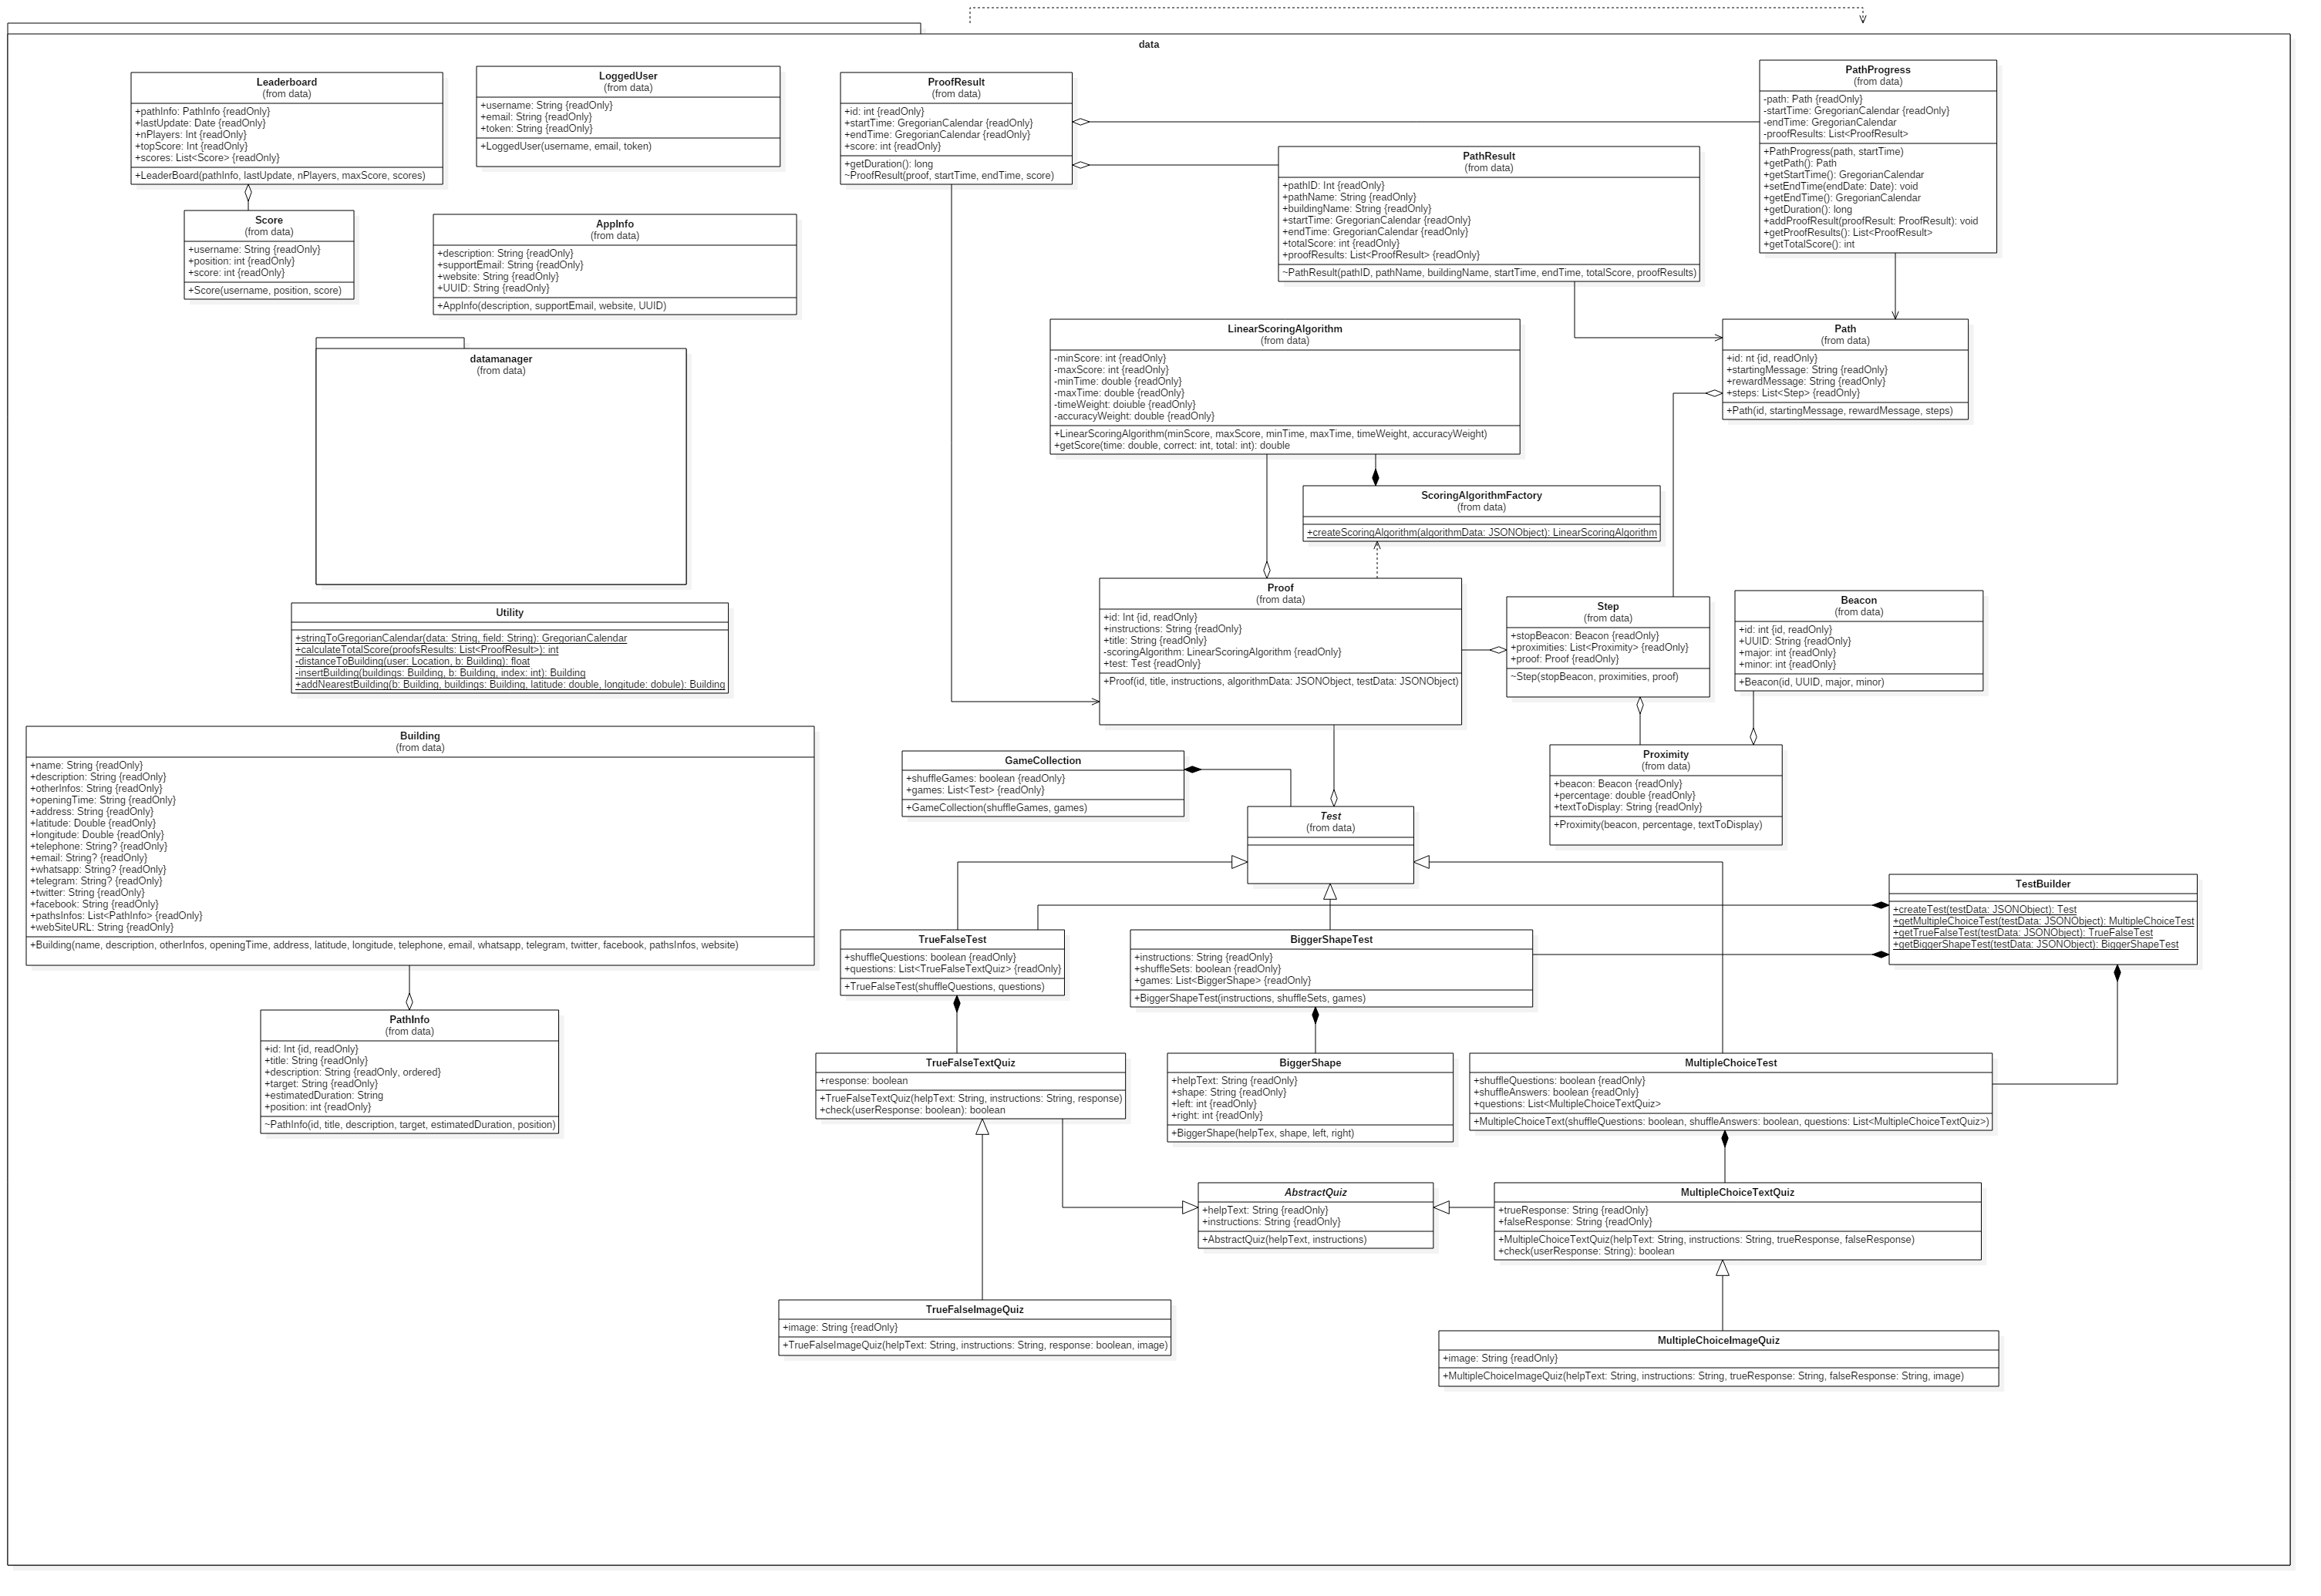
\includegraphics[scale=0.4]{img/package/png/client--data.png} 
\caption{Schema package client::data} 
 \end{figure} 
\compDescrizione{package per la gestione in locale dei dati}
\compPadre{client}
\begin{compPackageContenuti}
\item CLIPS::client::data::datamanager: componente che gestisce i dati in locale
\item CLIPS::client::data::urlrequest: componente che si occupa di effettuare le richieste al server
\end{compPackageContenuti}
\begin{compClassi} \\ 
\begin{classe}{CLIPS::client::data::AbstractImageQuiz}
\classeDescrizione{classe astratta per la creazione di quiz con immagine}
\classeUtilizzo{consente di creare un quiz con immagine}
\begin{classeRelazioni}
\classeRelazione{CLIPS::client::data}{AbstractQuiz}{interfaccia per la creazione delle classi astratte}\end{classeRelazioni}
\end{classe}\begin{classe}{CLIPS::client::data::AbstractQuiz}
\classeDescrizione{interfaccia per la creazione delle classi astratte}
\classeUtilizzo{permette di creare le classi astratte}
\end{classe}\begin{classe}{CLIPS::client::data::AbstractTextQuiz}
\classeDescrizione{classe astratta per la creazione di quiz con testo}
\classeUtilizzo{consente di creare un quiz con testo}
\begin{classeRelazioni}
\classeRelazione{CLIPS::client::data}{AbstractQuiz}{interfaccia per la creazione delle classi astratte}\end{classeRelazioni}
\end{classe}\begin{classe}{CLIPS::client::data::AppInfo}
\classeDescrizione{classe per la rappresentazione delle informazioni dell'applicazione}
\classeUtilizzo{permette di salvare le informazioni generali relative all'applicazione}
\end{classe}\begin{classe}{CLIPS::client::data::Beacon}
\classeDescrizione{classe che rappresenta un beacon in locale}
\classeUtilizzo{permette di salvere in locale le informazioni di un beacon}
\begin{classeAttributi}
\classeAttributo{id}{int}{rappresenta il codice identificativo}
\classeAttributo{major}{int}{rappresenta il parametro major di un beacon}
\classeAttributo{minor}{int}{rappresenta il parametro minor di un beacon}
\classeAttributo{UUID}{string}{rappresenta il codice UUID di un beacon}
\end{classeAttributi}
\begin{classeMetodi}
\classeMetodo{Beacon(id:int,UUID:string,major:int,minor:int)}{id, major, minor, UUID}{void}{costruttore della classe beacon}
\begin{classeMetodoArgomenti}
\classeMetodoArgomento{id}{int}{codice identificativo}
\classeMetodoArgomento{major}{int}{parametro major del beacon}
\classeMetodoArgomento{minor}{int}{parametro minor del beacon}
\classeMetodoArgomento{UUID}{string}{codice UUID}
\end{classeMetodoArgomenti}
\end{classeMetodi}
\end{classe}\begin{classe}{CLIPS::client::data::Building}
\classeDescrizione{classe che rappresenta un edificio}
\classeUtilizzo{permette di memorizzare i dati di un edificio in locale}
\begin{classeAttributi}
\classeAttributo{address}{string}{indica l'indirizzo dell'edificio}
\classeAttributo{description}{string}{rappresenta una breve descrizione dell'edificio}
\classeAttributo{email}{string}{rappresenta l'indirizzo email dell'edificio}
\classeAttributo{facebook}{string}{indica l'indirizzo facebook dell'edificio}
\classeAttributo{id}{int}{identifica l'edificio univocamente}
\classeAttributo{latitude}{double}{rappresenta la latitudine dell'edificio}
\classeAttributo{longitude}{double}{rappresenta la longitudine dell'edificio}
\classeAttributo{name}{string}{indica il nome dell'edificio}
\classeAttributo{openingTime}{void}{rappresenta gli orari di apertura dell'edificio}
\classeAttributo{otherInfos}{string}{contiene informazioni aggiuntive sull'edificio}
\classeAttributo{pathsInfos}{void}{fornisce informazioni sui percorsi dell'edificio}
\classeAttributo{telegram}{string}{rappresenta il contatto telegram dell'edificio}
\classeAttributo{telephone}{string}{indica il numero di telefono dell'edificio}
\classeAttributo{twitter}{string}{rappresenta l'indirizzo twitter dell'edificio}
\classeAttributo{webSiteURL}{string}{indica l'indirizzo web dell'edificio}
\classeAttributo{whatsapp}{string}{indica il contatto whatsapp dell'edificio}
\end{classeAttributi}
\begin{classeRelazioni}
\classeRelazione{CLIPS::client::data}{PathInfo}{classe che si occupa di salvare in locale le informazioni generali di un percorso}\end{classeRelazioni}
\end{classe}\begin{classe}{CLIPS::client::data::ConcreteMultipleChoice}
\classeDescrizione{classe che rappresenta un test a scelta multipla}
\classeUtilizzo{permette di creare un test a scelta multipla}
\begin{classeRelazioni}
\classeRelazione{CLIPS::client::data}{MultipleChoiceImage}{classe che rappresenta un test a scelta multipla con immagine}\classeRelazione{CLIPS::client::data}{MultipleChoiceText}{classe che rappresenta un test a scelta multipla con testo}\classeRelazione{CLIPS::client::data}{TestFactory}{interfaccia per costruire i test}\end{classeRelazioni}
\end{classe}\begin{classe}{CLIPS::client::data::ConcreteTrueFalse}
\classeDescrizione{classe che rappresenta un test true false}
\classeUtilizzo{permette di creare un test true false}
\begin{classeRelazioni}
\classeRelazione{CLIPS::client::data}{MultipleChoiceImage}{classe che rappresenta un test a scelta multipla con immagine}\classeRelazione{CLIPS::client::data}{TestFactory}{interfaccia per costruire i test}\classeRelazione{CLIPS::client::data}{TestFactory}{interfaccia per costruire i test}\classeRelazione{CLIPS::client::data}{TrueFalseImage}{classe che rappresenta un test true false con immagine}\end{classeRelazioni}
\end{classe}\begin{classe}{CLIPS::client::data::LeaderBoard}
\classeDescrizione{classe che rappresenta la classifica di un percorso}
\classeUtilizzo{consente di salvare i dati della classifica in locale}
\begin{classeRelazioni}
\classeRelazione{CLIPS::client::data}{Score}{classe che rappresenta il punteggio di un utente}\end{classeRelazioni}
\end{classe}\begin{classe}{CLIPS::client::data::LinearScoringAlgorithm}
\classeDescrizione{classe per calcolare il punteggio di una prova}
\classeUtilizzo{si occupa di calcolare il punteggio utilizzando un algoritmo lineare}
\begin{classeAttributi}
\classeAttributo{accuracyWeight}{double}{indica l'incidenza dell'accuratezza rispetto alla risposta}
\classeAttributo{maxScore}{int}{indica il punteggio massimo}
\classeAttributo{maxTime}{double}{indica il tempo massimo}
\classeAttributo{minScore}{int}{indica il punteggio minimo}
\classeAttributo{minTime}{double}{indica il tempo minimo}
\classeAttributo{timeWeight}{double}{indica l'incidenza del tempo nel calcolo del punteggio}
\end{classeAttributi}
\begin{classeMetodi}
\classeMetodo{getScore}{correct, total}{int}{fornisce il punteggio ottenuto nella prova}
\begin{classeMetodoArgomenti}
\classeMetodoArgomento{correct}{int}{indica il numero di risposte corrette}
\classeMetodoArgomento{total}{int}{*da aggiungere*}
\end{classeMetodoArgomenti}
\end{classeMetodi}
\end{classe}\begin{classe}{CLIPS::client::data::LoggedUser}
\classeDescrizione{classe che si occupa di memorizzare in locale i dati dell'utente loggato}
\classeUtilizzo{permette il salvataggio in locale dei dati di un utente loggato}
\end{classe}\begin{classe}{CLIPS::client::data::MultipleChoiceImage}
\classeDescrizione{classe che rappresenta un test a scelta multipla con immagine}
\classeUtilizzo{permette di creare un test a scelta multipla con immagine}
\begin{classeRelazioni}
\classeRelazione{CLIPS::client::data}{AbstractImageQuiz}{classe astratta per la creazione di quiz con immagine}\end{classeRelazioni}
\end{classe}\begin{classe}{CLIPS::client::data::MultipleChoiceText}
\classeDescrizione{classe che rappresenta un test a scelta multipla con testo}
\classeUtilizzo{permette di creare un test a scelta multipla con testo}
\begin{classeRelazioni}
\classeRelazione{CLIPS::client::data}{AbstractTextQuiz}{classe astratta per la creazione di quiz con testo}\end{classeRelazioni}
\end{classe}\begin{classe}{CLIPS::client::data::Path}
\classeDescrizione{classe che si occupa di salvare in locale i dati riguardanti un percorso}
\classeUtilizzo{permette di salvare i dati di un percorso in locale}
\begin{classeRelazioni}
\classeRelazione{CLIPS::client::data}{StepServer}{}\end{classeRelazioni}
\end{classe}\begin{classe}{CLIPS::client::data::PathInfo}
\classeDescrizione{classe che si occupa di salvare in locale le informazioni generali di un percorso}
\classeUtilizzo{consente di salvare in locale le informazioni generali di un percorso}
\end{classe}\begin{classe}{CLIPS::client::data::PathProgress}
\classeDescrizione{classe per il salvataggio in locale del progresso di un percorso}
\classeUtilizzo{permette di salvare in locale i risultati delle prove durante lo svolgimento del percorso}
\begin{classeRelazioni}
\classeRelazione{CLIPS::client::data}{Path}{classe che si occupa di salvare in locale i dati riguardanti un percorso}\end{classeRelazioni}
\end{classe}\begin{classe}{CLIPS::client::data::PathResult}
\classeDescrizione{classe che rappresenta i risultati di un percorso}
\classeUtilizzo{permette di salvare i dati di un percorso in locale}
\begin{classeRelazioni}
\classeRelazione{CLIPS::client::data}{Path}{classe che si occupa di salvare in locale i dati riguardanti un percorso}\end{classeRelazioni}
\end{classe}\begin{classe}{CLIPS::client::data::Proof}
\classeDescrizione{classe che rappresenta una prova del percorso}
\classeUtilizzo{salva in locale i dati della prova da far visualizzare all'utente}
\begin{classeRelazioni}
\classeRelazione{CLIPS::client::data}{LinearScoringAlgorithm}{classe per calcolare il punteggio di una prova}\classeRelazione{CLIPS::client::data}{ScoringAlgorithmFactory}{classe base per la creazione degli algoritmi}\classeRelazione{CLIPS::client::data}{TestFactory}{interfaccia per costruire i test}\end{classeRelazioni}
\end{classe}\begin{classe}{CLIPS::client::data::ProofResult}
\classeDescrizione{classe che rappresenta il risultato di una prova}
\classeUtilizzo{permette di salvare in locale il risultato di una prova}
\begin{classeRelazioni}
\classeRelazione{CLIPS::client::data}{PathProgress}{classe per il salvataggio in locale del progresso di un percorso}\classeRelazione{CLIPS::client::data}{PathResult}{classe che rappresenta i risultati di un percorso}\classeRelazione{CLIPS::client::data}{Proof}{classe che rappresenta una prova del percorso}\end{classeRelazioni}
\end{classe}\begin{classe}{CLIPS::client::data::Proximity}
\classeDescrizione{classe che rappresenta in locale un beacon indicato alla segnalazione della distanza dalla prossima prova}
\classeUtilizzo{consente di salvare un beacon e la sua distanza dal beacon della prossima prova}
\begin{classeRelazioni}
\classeRelazione{CLIPS::client::data}{Building}{classe che rappresenta un edificio}\end{classeRelazioni}
\end{classe}\begin{classe}{CLIPS::client::data::Quiz}
\classeDescrizione{classe che rappresenta un quiz}
\classeUtilizzo{viene utilizzata per salvare i dati del quiz}
\begin{classeAttributi}
\classeAttributo{playerHasOneAttempt}{bool}{indica se il giocatore ha un solo tentativo per il quiz}
\classeAttributo{qas}{void}{*da aggiungere*}
\end{classeAttributi}
\begin{classeRelazioni}
\classeRelazione{CLIPS::client::data}{Test}{classe che rappresenta un test}\end{classeRelazioni}
\end{classe}\begin{classe}{CLIPS::client::data::Score}
\classeDescrizione{classe che rappresenta il punteggio di un utente}
\classeUtilizzo{permette di memorizzare i dati del punteggio di un utente}
\end{classe}\begin{classe}{CLIPS::client::data::ScoringAlgorithmFactory}
\classeDescrizione{classe base per la creazione degli algoritmi}
\classeUtilizzo{fornisce il metodo per la creazione di algoritmi per il calcolo dei punteggi}
\begin{classeMetodi}
\classeMetodo{createScoringAlgorithm}{algorithmData}{void}{si occupa di creare l'algoritmo per calcolare il punteggio}
\begin{classeMetodoArgomenti}
\classeMetodoArgomento{algorithmData}{void}{*da aggiungere*}
\end{classeMetodoArgomenti}
\end{classeMetodi}
\begin{classeRelazioni}
\classeRelazione{CLIPS::client::data}{LinearScoringAlgorithm}{classe per calcolare il punteggio di una prova}\end{classeRelazioni}
\end{classe}\begin{classe}{CLIPS::client::data::Step}
\classeDescrizione{classe che rappresenta in locale lo spostamento da una prova a quella successiva}
\classeUtilizzo{permette di salvare in locale le informazioni che rappresentano la ricerca della nuova prova}
\end{classe}\begin{classe}{CLIPS::client::data::Test}
\classeDescrizione{classe che rappresenta un test}
\classeUtilizzo{vengono salvati in locale i dati del test}
\begin{classeRelazioni}
\classeRelazione{CLIPS::client::data}{AbstractQuiz}{interfaccia per la creazione delle classi astratte}\classeRelazione{CLIPS::client::data}{Proof}{classe che rappresenta una prova del percorso}\classeRelazione{CLIPS::client::data}{TestFactory}{interfaccia per costruire i test}\end{classeRelazioni}
\end{classe}\begin{classe}{CLIPS::client::data::TestFactory}
\classeDescrizione{interfaccia per costruire i test}
\classeUtilizzo{viene utilizzata per costruire i test concreti}
\begin{classeRelazioni}
\classeRelazione{CLIPS::client::data}{Test}{classe che rappresenta un test}\end{classeRelazioni}
\end{classe}\begin{classe}{CLIPS::client::data::TrueFalseImage}
\classeDescrizione{classe che rappresenta un test true false con immagine}
\classeUtilizzo{permette di creare un test true false con immagine}
\begin{classeRelazioni}
\classeRelazione{CLIPS::client::data}{AbstractImageQuiz}{classe astratta per la creazione di quiz con immagine}\end{classeRelazioni}
\end{classe}\begin{classe}{CLIPS::client::data::TrueFalseText}
\classeDescrizione{classe che rappresenta un test true false con testo}
\classeUtilizzo{permette di creare un test true false con testo}
\begin{classeRelazioni}
\classeRelazione{CLIPS::client::data}{AbstractTextQuiz}{classe astratta per la creazione di quiz con testo}\end{classeRelazioni}
\end{classe}\end{compClassi}
\end{componente}
\begin{componente}{CLIPS::client::data::datamanager}
\begin{figure}[h!] 
\centering 
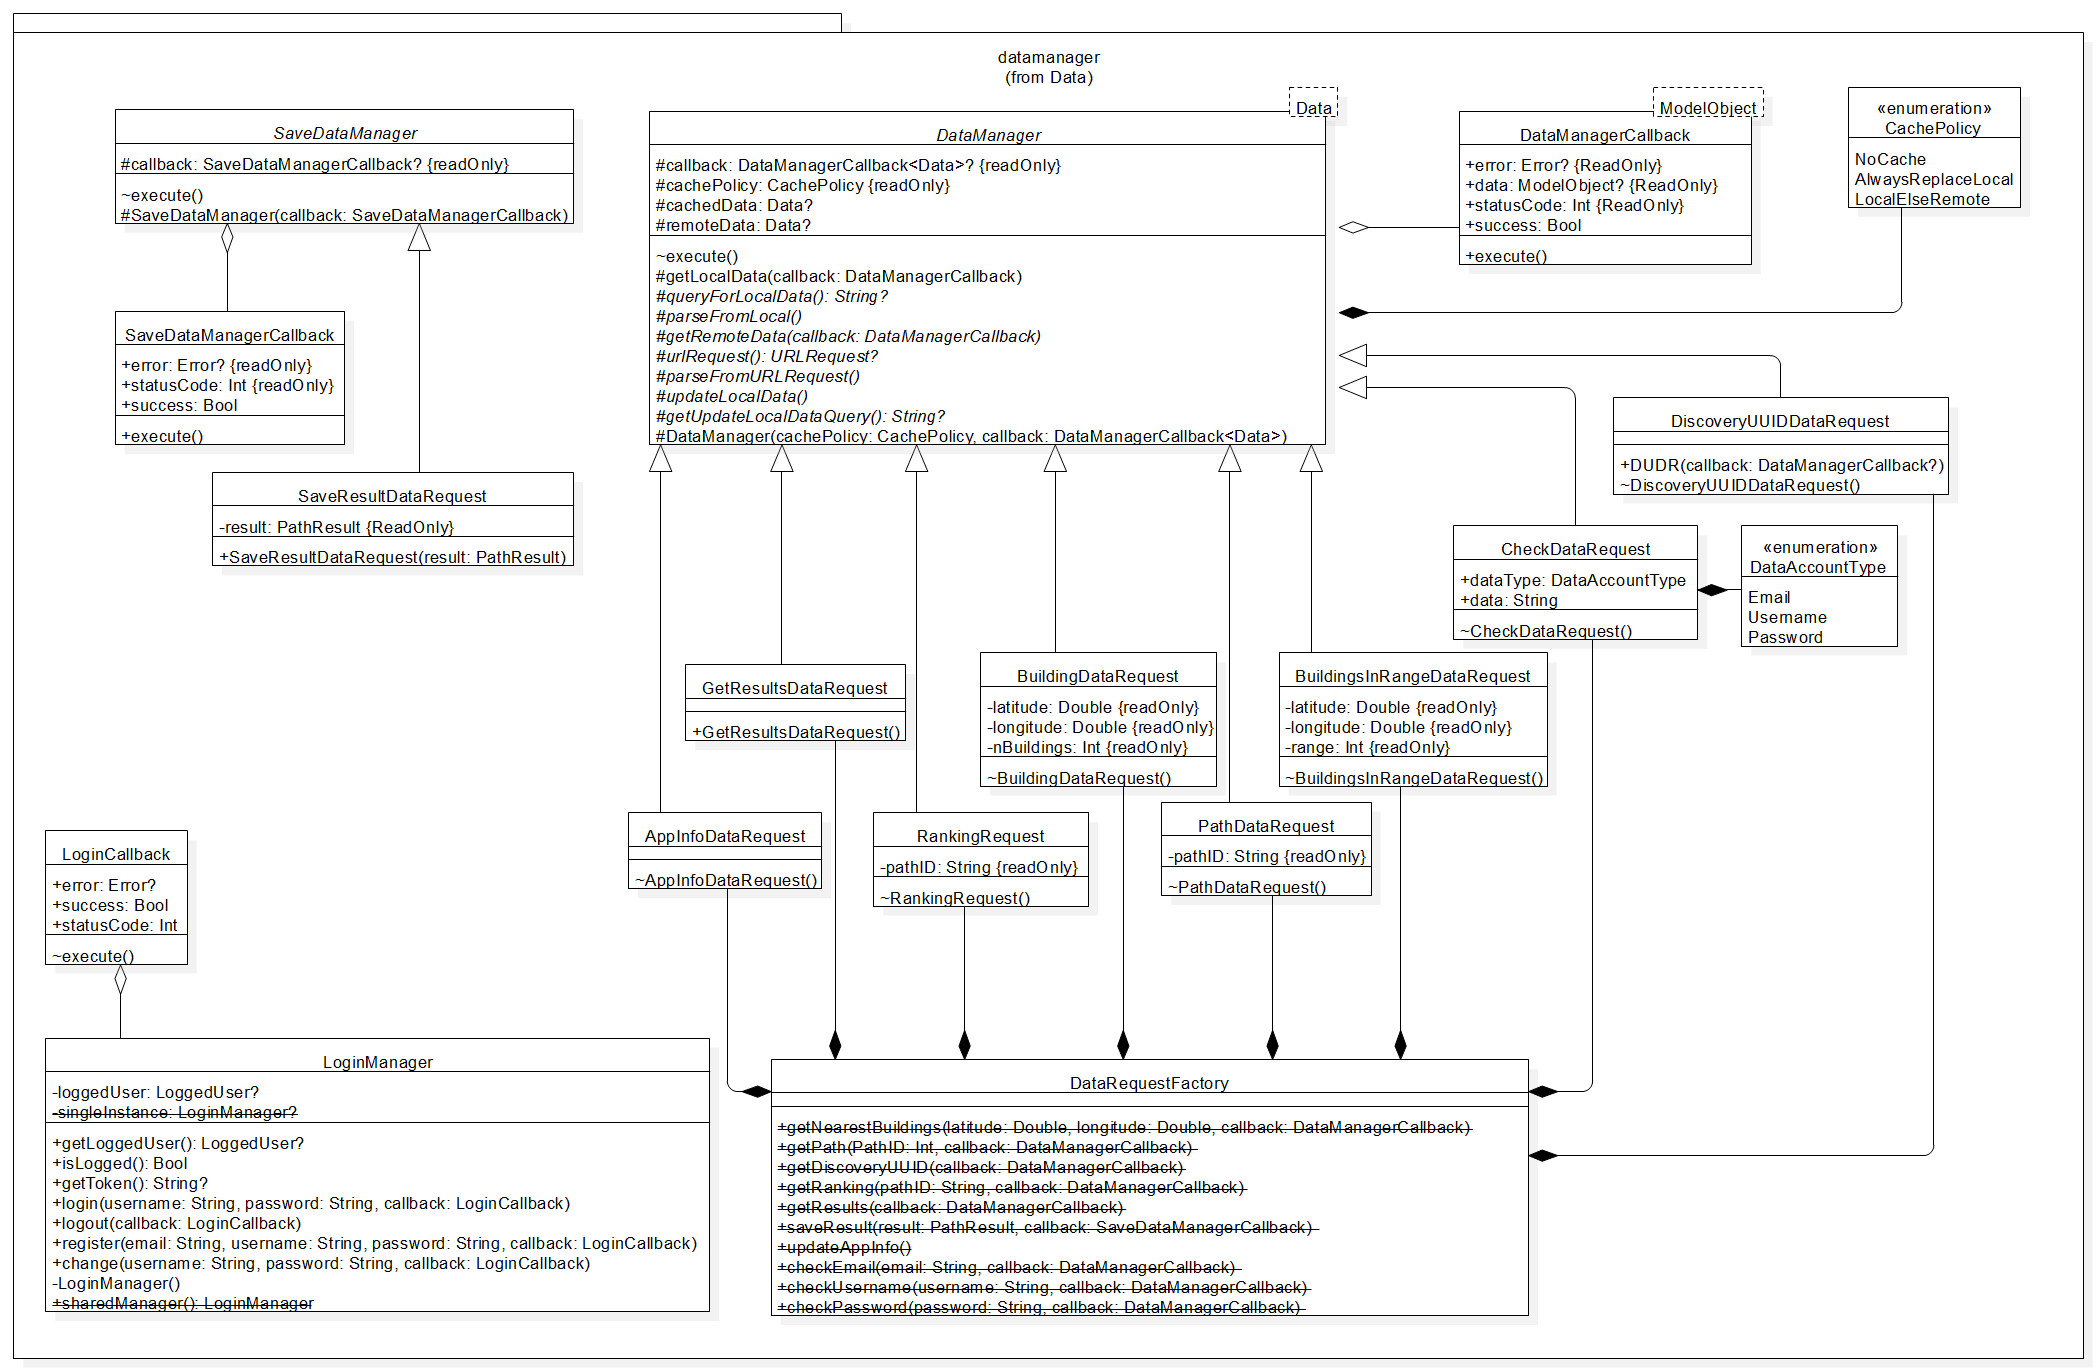
\includegraphics[scale=0.4]{img/package/png/client--datamanager.png} 
\caption{Schema package client::datamanager} 
 \end{figure} 
\compDescrizione{componente che gestisce i dati in locale}
\compPadre{data}
\begin{compClassi} \\ 
\begin{classe}{CLIPS::client::data::datamanager::AppInfoDataRequest}
\classeDescrizione{classe concreta che gestisce le richieste dei dati sulle info dell'app}
\classeUtilizzo{permette di ottenere i dati sulle informazioni dell'app}
\begin{classeRelazioni}
\classeRelazione{CLIPS::client::data::datamanager}{DataManager}{classe astratta per la gestione dello scambio di richieste e dati tra client e server}\end{classeRelazioni}
\end{classe}\begin{classe}{CLIPS::client::data::datamanager::BuildingDataRequest}
\classeDescrizione{classe concreta che gestisce le richieste dei dati sugli edifici}
\classeUtilizzo{permette di ottenere i dati sugli edifici}
\begin{classeRelazioni}
\classeRelazione{CLIPS::client::data::datamanager}{DataManager}{classe astratta per la gestione dello scambio di richieste e dati tra client e server}\end{classeRelazioni}
\end{classe}\begin{classe}{CLIPS::client::data::datamanager::BuildingsInRangeDataRequest}
\classeDescrizione{classe concreta che gestisce le richieste dei dati sugli edifici nel raggio inserito}
\classeUtilizzo{permette di ottenere i dati sugli edifici nel raggio inserito}
\begin{classeRelazioni}
\classeRelazione{CLIPS::client::data::datamanager}{DataManager}{classe astratta per la gestione dello scambio di richieste e dati tra client e server}\end{classeRelazioni}
\end{classe}\begin{classe}{CLIPS::client::data::datamanager::CachePolicy}
\classeDescrizione{classe che determina i tipi di politica della cache}
\classeUtilizzo{determina i tipi di politica della cache}
\end{classe}\begin{classe}{CLIPS::client::data::datamanager::CheckDataRequest}
\classeDescrizione{classe concreta che gestisce le richieste di check sui dati}
\classeUtilizzo{permette di ottenere il check sui dati}
\begin{classeRelazioni}
\classeRelazione{CLIPS::client::data::datamanager}{DataAccountType}{classe che determina i tipi di dato di un account}\classeRelazione{CLIPS::client::data::datamanager}{DataManager}{classe astratta per la gestione dello scambio di richieste e dati tra client e server}\end{classeRelazioni}
\end{classe}\begin{classe}{CLIPS::client::data::datamanager::DataAccountType}
\classeDescrizione{classe che determina i tipi di dato di un account}
\classeUtilizzo{determina i tipi di dato in un'account}
\end{classe}\begin{classe}{CLIPS::client::data::datamanager::DataManager}
\classeDescrizione{classe astratta per la gestione dello scambio di richieste e dati tra client e server}
\classeUtilizzo{permette lo scambio di dati tra server e client}
\begin{classeRelazioni}
\classeRelazione{CLIPS::client::data::datamanager}{CachePolicy}{classe che determina i tipi di politica della cache}\classeRelazione{CLIPS::client::data::datamanager}{DataManagerCallback}{classe che gestisce le callback effettuate dal data manager}\end{classeRelazioni}
\end{classe}\begin{classe}{CLIPS::client::data::datamanager::DataManagerCallback}
\classeDescrizione{classe che gestisce le callback effettuate dal data manager}
\classeUtilizzo{permette di effettuare le callback al data manager}
\end{classe}\begin{classe}{CLIPS::client::data::datamanager::DataRequestFactory}
\classeDescrizione{classe che effettua le richieste al server}
\classeUtilizzo{permette di effettuare richieste al server}
\begin{classeRelazioni}
\classeRelazione{CLIPS::client::data::datamanager}{AppInfoDataRequest}{classe concreta che gestisce le richieste dei dati sulle info dell'app}\classeRelazione{CLIPS::client::data::datamanager}{BuildingDataRequest}{classe concreta che gestisce le richieste dei dati sugli edifici}\classeRelazione{CLIPS::client::data::datamanager}{BuildingsInRangeDataRequest}{classe concreta che gestisce le richieste dei dati sugli edifici nel raggio inserito}\classeRelazione{CLIPS::client::data::datamanager}{CheckDataRequest}{classe concreta che gestisce le richieste di check sui dati}\classeRelazione{CLIPS::client::data::datamanager}{DiscoveryUUIDDataRequest}{classe concreta che gestisce le richieste di ricerca di un beacon}\classeRelazione{CLIPS::client::data::datamanager}{GetResultsDataRequest}{classe concreta che gestisce le richieste dei dati dei risultati}\classeRelazione{CLIPS::client::data::datamanager}{PathDataRequest}{classe concreta che gestisce le richieste dei dati sui percorsi}\classeRelazione{CLIPS::client::data::datamanager}{RankingRequest}{classe concreta che gestisce le richieste dei dati della classifica}\end{classeRelazioni}
\end{classe}\begin{classe}{CLIPS::client::data::datamanager::DiscoveryUUIDDataRequest}
\classeDescrizione{classe concreta che gestisce le richieste di ricerca di un beacon}
\classeUtilizzo{permette di ottenere gli UUID di un beacon}
\begin{classeRelazioni}
\classeRelazione{CLIPS::client::data::datamanager}{DataManager}{classe astratta per la gestione dello scambio di richieste e dati tra client e server}\end{classeRelazioni}
\end{classe}\begin{classe}{CLIPS::client::data::datamanager::GetResultsDataRequest}
\classeDescrizione{classe concreta che gestisce le richieste dei dati dei risultati}
\classeUtilizzo{permette di ottenere i dati dei risultati}
\begin{classeRelazioni}
\classeRelazione{CLIPS::client::data::datamanager}{DataManager}{classe astratta per la gestione dello scambio di richieste e dati tra client e server}\end{classeRelazioni}
\end{classe}\begin{classe}{CLIPS::client::data::datamanager::LoginCallback}
\classeDescrizione{classe che gestisce le callback per il login}
\classeUtilizzo{permette di effettuare le callback per il login}
\end{classe}\begin{classe}{CLIPS::client::data::datamanager::LoginManager}
\classeDescrizione{classe che gestisce il controllo del login tra view e server}
\classeUtilizzo{permette di effettuare il login}
\begin{classeRelazioni}
\classeRelazione{CLIPS::client::data::datamanager}{LoginCallback}{classe che gestisce le callback per il login}\end{classeRelazioni}
\end{classe}\begin{classe}{CLIPS::client::data::datamanager::PathDataRequest}
\classeDescrizione{classe concreta che gestisce le richieste dei dati sui percorsi}
\classeUtilizzo{permette di ottenere i dati sui percorsi}
\begin{classeRelazioni}
\classeRelazione{CLIPS::client::data::datamanager}{DataManager}{classe astratta per la gestione dello scambio di richieste e dati tra client e server}\end{classeRelazioni}
\end{classe}\begin{classe}{CLIPS::client::data::datamanager::RankingRequest}
\classeDescrizione{classe concreta che gestisce le richieste dei dati della classifica}
\classeUtilizzo{permette di ottenere i dati della classifica}
\begin{classeRelazioni}
\classeRelazione{CLIPS::client::data::datamanager}{DataManager}{classe astratta per la gestione dello scambio di richieste e dati tra client e server}\end{classeRelazioni}
\end{classe}\begin{classe}{CLIPS::client::data::datamanager::SaveDataManager}
\classeDescrizione{classe astratta per il salvataggio di dati nel server}
\classeUtilizzo{permette di effettuare il salvataggio dei dati nel server}
\begin{classeRelazioni}
\classeRelazione{CLIPS::client::data::datamanager}{SaveDataManagerCallback}{classe che si occupa di effettuare le callback per il salvataggio dei dati nel server}\end{classeRelazioni}
\end{classe}\begin{classe}{CLIPS::client::data::datamanager::SaveDataManagerCallback}
\classeDescrizione{classe che si occupa di effettuare le callback per il salvataggio dei dati nel server}
\classeUtilizzo{permette di effettuare i callback}
\end{classe}\begin{classe}{CLIPS::client::data::datamanager::SaveResultDataRequest}
\classeDescrizione{classe concreta che effettua le richieste per salvare i dati}
\classeUtilizzo{permette di ottenere la locazione per il salvataggio dei dati}
\begin{classeRelazioni}
\classeRelazione{CLIPS::client::data::datamanager}{SaveDataManager}{classe astratta per il salvataggio di dati nel server}\end{classeRelazioni}
\end{classe}\end{compClassi}
\end{componente}
\begin{componente}{CLIPS::client::data::urlrequest}
\begin{figure}[h!] 
\centering 
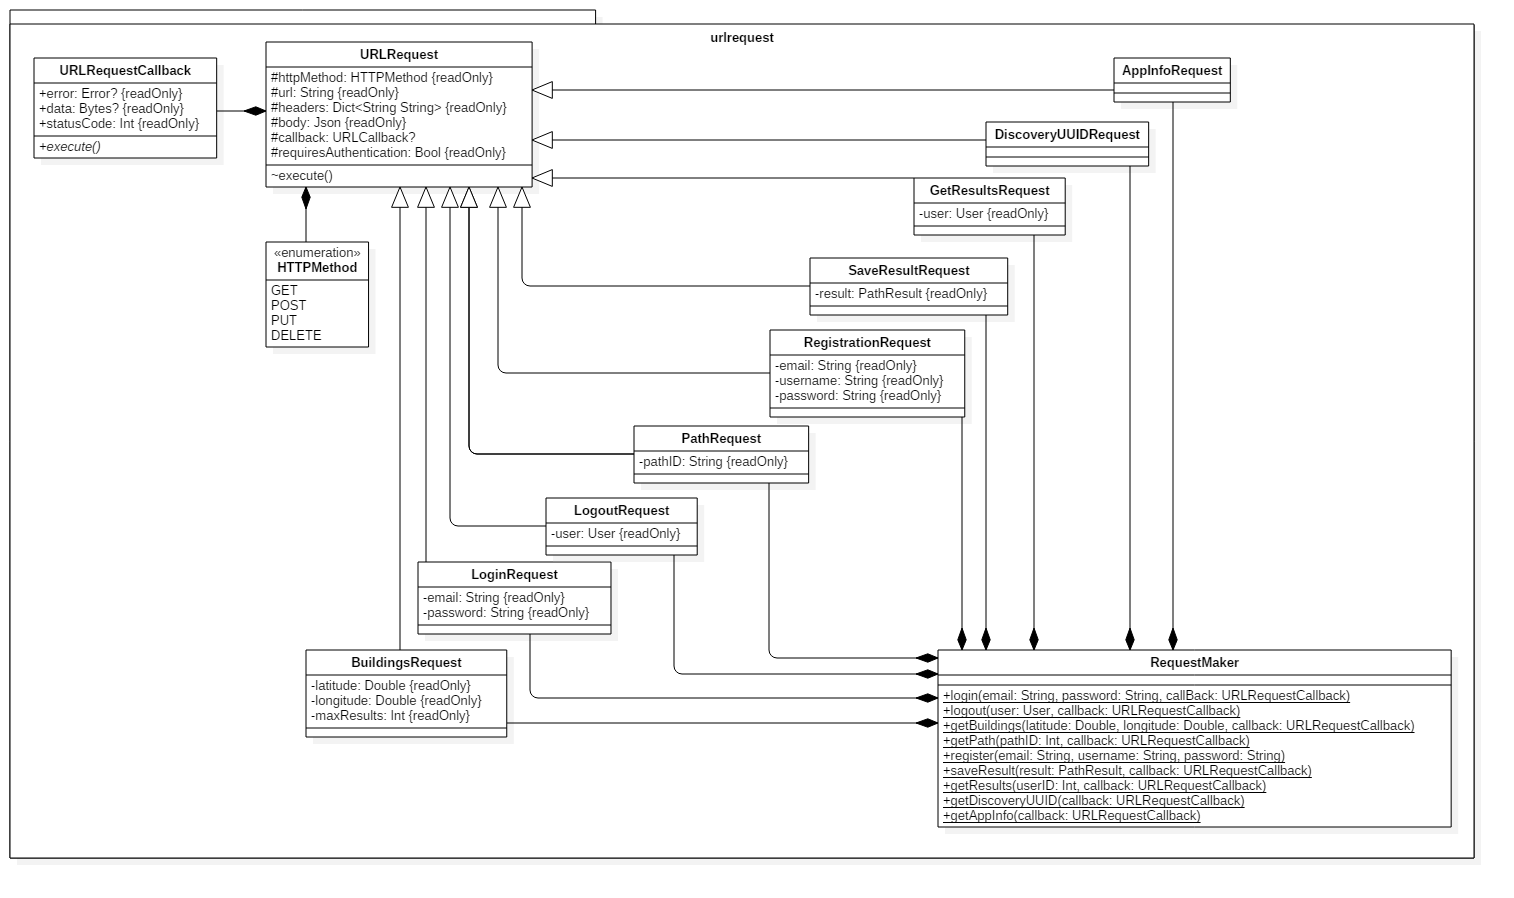
\includegraphics[scale=0.4]{img/package/png/client--urlrequest.png} 
\caption{Schema package client::urlrequest} 
 \end{figure} 
\compDescrizione{componente che si occupa di effettuare le richieste al server}
\compPadre{data}
\begin{compClassi} \\ 
\begin{classe}{CLIPS::client::data::urlrequest::AppInfoRequest}
\classeDescrizione{classe per la richiesta di dati sulle info dell'app}
\classeUtilizzo{permette di effettuare una richiesta al server di dati sulle info dell'app}
\end{classe}\begin{classe}{CLIPS::client::data::urlrequest::BuildingRequest}
\classeDescrizione{classe per la richiesta di dati sugli edifici}
\classeUtilizzo{permette di effettuare una richiesta al server di dati sugli edifici}
\end{classe}\begin{classe}{CLIPS::client::data::urlrequest::DiscoveryUUIDRequest}
\classeDescrizione{classe per la richiesta di un ricerca di un beacon}
\classeUtilizzo{permette di effettuare richieste di ricerca di un beacon}
\end{classe}\begin{classe}{CLIPS::client::data::urlrequest::GetResultsRequest}
\classeDescrizione{classe per la richiesta di risultati}
\classeUtilizzo{permette di effettuare richiest di dati dei risultati}
\end{classe}\begin{classe}{CLIPS::client::data::urlrequest::HTTPMethod}
\classeDescrizione{classe che dichiara i metodi per le chiamate REST}
\classeUtilizzo{dichiara i metodi per le chiamate REST}
\end{classe}\begin{classe}{CLIPS::client::data::urlrequest::LoginRequest}
\classeDescrizione{classe per la richiesta di login}
\classeUtilizzo{permette di effettuare una richiesta di login}
\end{classe}\begin{classe}{CLIPS::client::data::urlrequest::LogoutRequest}
\classeDescrizione{classe per la richiesta di logout}
\classeUtilizzo{permette di effettuare una richiesta di logout}
\end{classe}\begin{classe}{CLIPS::client::data::urlrequest::PathRequest}
\classeDescrizione{classe per la richiesta di dati sui percorsi}
\classeUtilizzo{permette di richiedere dati sui percorsi}
\end{classe}\begin{classe}{CLIPS::client::data::urlrequest::RegistrationRequest}
\classeDescrizione{classe per la richiesta di registrazione}
\classeUtilizzo{permette di effettuare una richiesta di registrazione}
\end{classe}\begin{classe}{CLIPS::client::data::urlrequest::RequestMaker}
\classeDescrizione{classe per la costruzione e l'invio di richieste al server}
\classeUtilizzo{permette la costruzione e l'invio di richieste al server}
\begin{classeRelazioni}
\classeRelazione{CLIPS::client::data::urlrequest}{AppInfoRequest}{classe per la richiesta di dati sulle info dell'app}\classeRelazione{CLIPS::client::data::urlrequest}{BuildingRequest}{classe per la richiesta di dati sugli edifici}\classeRelazione{CLIPS::client::data::urlrequest}{DiscoveryUUIDRequest}{classe per la richiesta di un ricerca di un beacon}\classeRelazione{CLIPS::client::data::urlrequest}{GetResultsRequest}{classe per la richiesta di risultati}\classeRelazione{CLIPS::client::data::urlrequest}{LoginRequest}{classe per la richiesta di login}\classeRelazione{CLIPS::client::data::urlrequest}{LogoutRequest}{classe per la richiesta di logout}\classeRelazione{CLIPS::client::data::urlrequest}{PathRequest}{classe per la richiesta di dati sui percorsi}\classeRelazione{CLIPS::client::data::urlrequest}{RegistrationRequest}{classe per la richiesta di registrazione}\classeRelazione{CLIPS::client::data::urlrequest}{SaveResultRequest}{classe per la richiesta di salvataggio di un risultato}\end{classeRelazioni}
\end{classe}\begin{classe}{CLIPS::client::data::urlrequest::SaveResultRequest}
\classeDescrizione{classe per la richiesta di salvataggio di un risultato}
\classeUtilizzo{permette di effettuare una richiesta di salvataggio di un risultato}
\end{classe}\begin{classe}{CLIPS::client::data::urlrequest::URLRequest}
\classeDescrizione{classe che si occupa delle richieste dell'URL al server}
\classeUtilizzo{permette di richiedere l'URL interessato}
\begin{classeRelazioni}
\classeRelazione{CLIPS::client::data::urlrequest}{HTTPMethod}{classe che dichiara i metodi per le chiamate REST}\classeRelazione{CLIPS::client::data::urlrequest}{URLRequestCallback}{classe che gestisce le callback per le richieste di URL}\end{classeRelazioni}
\end{classe}\begin{classe}{CLIPS::client::data::urlrequest::URLRequestCallback}
\classeDescrizione{classe che gestisce le callback per le richieste di URL}
\classeUtilizzo{permette di effettuare al URLRequest di effettuare delle callback}
\end{classe}\end{compClassi}
\end{componente}
\begin{componente}{CLIPS::client::location}
\begin{figure}[h!] 
\centering 
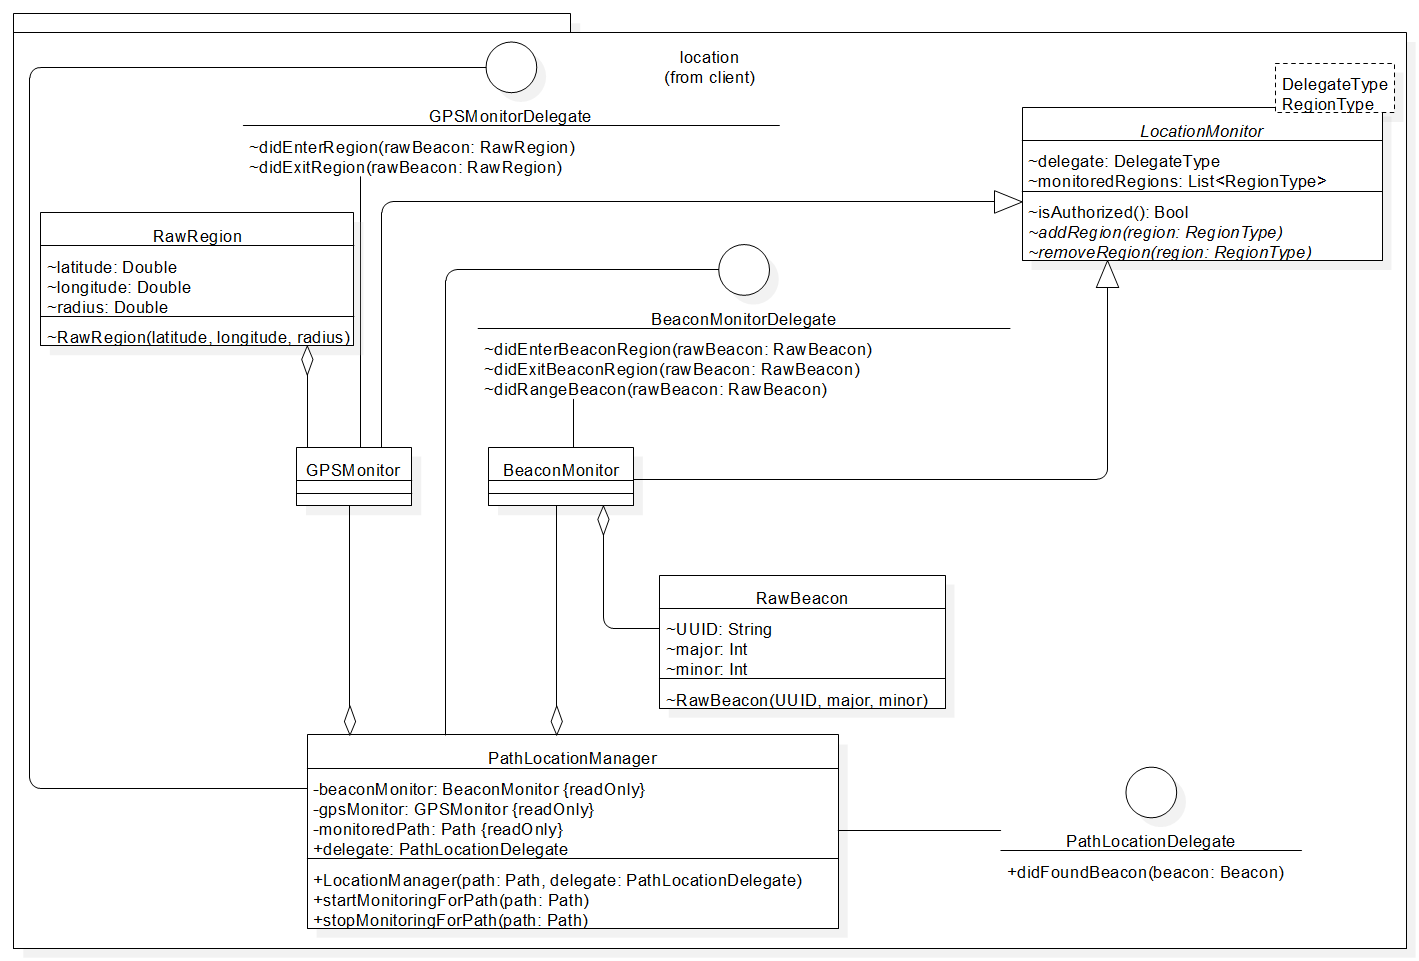
\includegraphics[scale=0.4]{img/package/png/client--location.png} 
\caption{Schema package client::location} 
 \end{figure} 
\compDescrizione{componente che gestisce l'individuazione e la lettura dei beacon}
\compPadre{client}
\begin{compClassi} \\ 
\begin{classe}{CLIPS::client::location::BeaconMonitor}
\classeDescrizione{classe che si occupa di monitorare la scoperta di nuovi beacon e l'allontanamento da beacon presenti}
\classeUtilizzo{PathLocationManager ne crea un'istanza e imposta se stesso come il suo delegate per essere notificato quando nuovi beacon entrano nel raggio del dispositivo}
\begin{classeRelazioni}
\classeRelazione{CLIPS::client::location}{BeaconMonitorDelegate}{interfaccia che devono implementare le classi che desiderano essere notificate dal BeaconMonitor}\classeRelazione{CLIPS::client::location}{LocationMonitor<DelegateType,RegionType>}{gli oggetti della classe LocationMonitor si occupano di monitorare quando il dispositivo entra od esce da una regione di tipo RegionType e notificano di ci� un oggetto di tipo DelegateType}\classeRelazione{CLIPS::client::location}{RawRegion}{oggetto che rappresenta una regione geografica circolare}\end{classeRelazioni}
\end{classe}\begin{classe}{CLIPS::client::location::BeaconMonitorDelegate}
\classeDescrizione{interfaccia che devono implementare le classi che desiderano essere notificate dal BeaconMonitor}
\classeUtilizzo{le classi che desiderano essere informate quando vengono scoperti nuovi beacon o quando un beacon noto esce dal raggio del dispositivo devono implementare questa interfaccia per permettere al BeaconMonitor di notificarle}
\end{classe}\begin{classe}{CLIPS::client::location::GPSMonitor}
\classeDescrizione{classe che si occupa di monitorare l'ingresso o l'uscita in una regione geografica registrata}
\classeUtilizzo{PathLocationManager ne può creare un'istanza e può impostare se stesso come il suo delegate per essere notificato quando l'utente entra od esce da una regione geografica registrata}
\begin{classeRelazioni}
\classeRelazione{CLIPS::client::location}{GPSMonitorDelegate}{interfaccia per segnalare gli eventi della classe GPSMonitor}\classeRelazione{CLIPS::client::location}{LocationMonitor<DelegateType,RegionType>}{gli oggetti della classe LocationMonitor si occupano di monitorare quando il dispositivo entra od esce da una regione di tipo RegionType e notificano di ci� un oggetto di tipo DelegateType}\end{classeRelazioni}
\end{classe}\begin{classe}{CLIPS::client::location::GPSMonitorDelegate}
\classeDescrizione{interfaccia per segnalare gli eventi della classe GPSMonitor}
\classeUtilizzo{si occupa di fornire i metodi necessari alla classe GPSMonitor}
\begin{classeRelazioni}
\classeRelazione{CLIPS::client::location}{GPSMonitor}{classe che si occupa di monitorare l'ingresso o l'uscita in una regione geografica registrata}\classeRelazione{CLIPS::client::location}{PathLocationManager}{classe che si occupa di gestire gli eventi legati alla posizione di un determinato percorso}\end{classeRelazioni}
\end{classe}\begin{classe}{CLIPS::client::location::LocationMonitor<DelegateType,RegionType>}
\classeDescrizione{gli oggetti della classe LocationMonitor si occupano di monitorare quando il dispositivo entra od esce da una regione di tipo RegionType e notificano di ci� un oggetto di tipo DelegateType}
\classeUtilizzo{le classi BeaconMonitor e GPSMonitor sono sottoclassi che monitorano rispettivamente delle regioni di tipo RawBeacon e RawRegion ed entrambe notificano un oggetto di tipo PathLocationManager}
\end{classe}\begin{classe}{CLIPS::client::location::PathLocationDelegate}
\classeDescrizione{interfaccia che devono implementare le classi che desiderano essere notificate quando il PathLocationManager rileva un beacon}
\classeUtilizzo{interfaccia implementata da PathProgress che desidera essere notificato quando PathLocationManager rileva un beacon di quelli appartenenti al percorso (Path) in corso}
\end{classe}\begin{classe}{CLIPS::client::location::PathLocationManager}
\classeDescrizione{classe che si occupa di gestire gli eventi legati alla posizione di un determinato percorso}
\classeUtilizzo{un oggetto di tipo PathLocationManager viene creato dal PathProgress che gli fornisce i dati sui beacon presenti nel percorso (che dovranno quindi essere monitorati) e imposta se stesso come delegate, per essere notificato di eventuali beacon che entrano/escono dal raggio del dispositivo}
\begin{classeRelazioni}
\classeRelazione{CLIPS::client::location}{BeaconMonitor}{classe che si occupa di monitorare la scoperta di nuovi beacon e l'allontanamento da beacon presenti}\classeRelazione{CLIPS::client::location}{BeaconMonitorDelegate}{interfaccia che devono implementare le classi che desiderano essere notificate dal BeaconMonitor}\classeRelazione{CLIPS::client::location}{GPSMonitor}{classe che si occupa di monitorare l'ingresso o l'uscita in una regione geografica registrata}\classeRelazione{CLIPS::client::location}{PathLocationDelegate}{interfaccia che devono implementare le classi che desiderano essere notificate quando il PathLocationManager rileva un beacon}\end{classeRelazioni}
\end{classe}\begin{classe}{CLIPS::client::location::RawBeacon}
\classeDescrizione{oggetto che rappresenta un Beacon: nonostante i campi siano simili alla classe \'Beacon\' il fatto che siano di tipi diversi enfatizza la differenza che c'è tra un Beacon (proveniente dal server e appartenente ad un percorso) e un RawBeacon (un oggetto monitorabile dalla classe BeaconMonitor)}
\classeUtilizzo{quando il PathLocationManager riceve un path, a partire dai suoi Beacon crea i necessari oggetti RawBeacon e chiede al proprio BeaconManager di monitorarli}
\end{classe}\begin{classe}{CLIPS::client::location::RawRegion}
\classeDescrizione{oggetto che rappresenta una regione geografica circolare}
\classeUtilizzo{utilizzata dal LocationManager per descrivere una regione geografica circolare}
\end{classe}\end{compClassi}
\end{componente}
\begin{componente}{CLIPS::client::pathprogress}
\begin{figure}[h!] 
\centering 
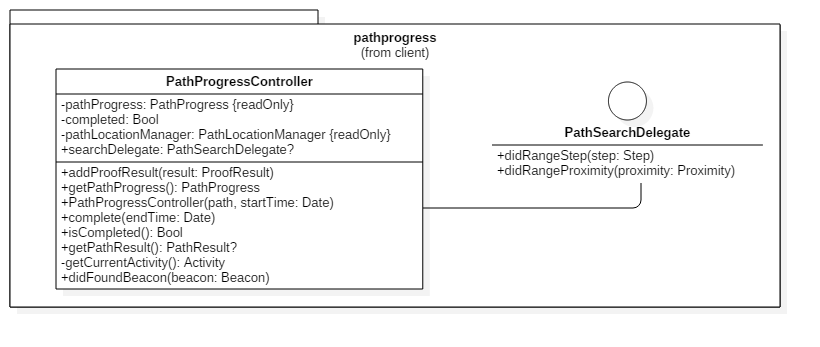
\includegraphics[scale=0.4]{img/package/png/client--pathprogress.png} 
\caption{Schema package client::pathprogress} 
 \end{figure} 
\compDescrizione{componente che gestisce i dati del percorso e salva i risultati ottenuti nelle prove mentre si sta giocando}
\compPadre{client}
\begin{compClassi} \\ 
\begin{classe}{CLIPS::client::pathprogress::PathProgressController}
\classeDescrizione{classe che gestisce l'avanzamento di un percorso}
\classeUtilizzo{permette di gestire i dati dell'avanzamento di un percorso}
\begin{classeRelazioni}
\classeRelazione{CLIPS::client::pathprogress}{PathSearchDelegate}{interfaccia per le funzioni di ricerca di un beacon in un percorso}\end{classeRelazioni}
\end{classe}\begin{classe}{CLIPS::client::pathprogress::PathSearchDelegate}
\classeDescrizione{interfaccia per le funzioni di ricerca di un beacon in un percorso}
\classeUtilizzo{permette di gestire la ricerca di un beacon}
\begin{classeRelazioni}
\classeRelazione{CLIPS::client::pathprogress}{PathProgressController}{classe che gestisce l'avanzamento di un percorso}\end{classeRelazioni}
\end{classe}\end{compClassi}
\end{componente}
\begin{componente}{CLIPS::client::viewcontroller}
\begin{figure}[h!] 
\centering 
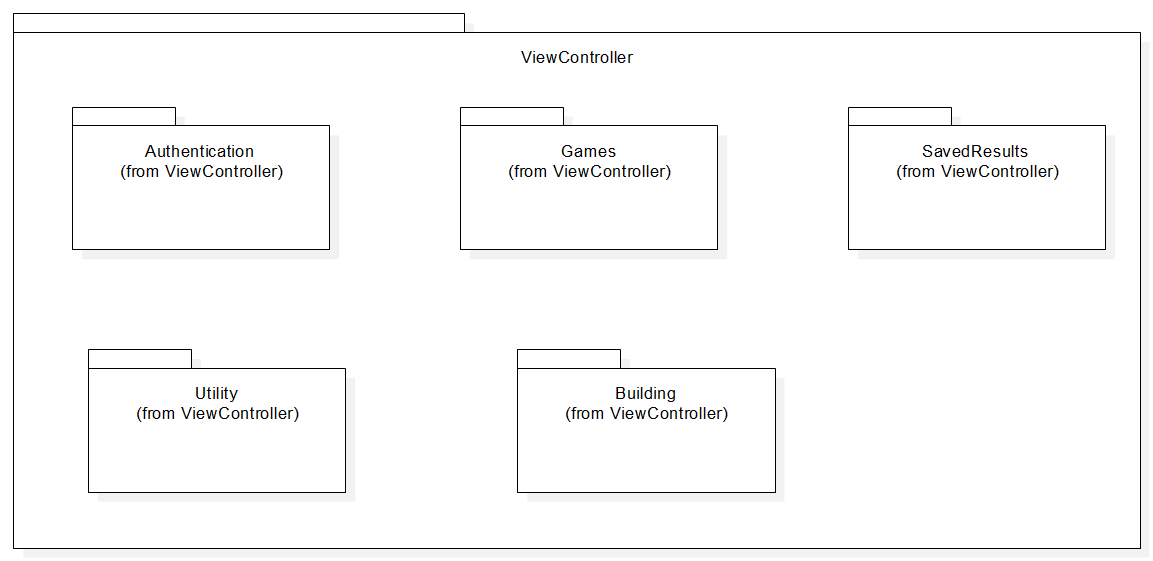
\includegraphics[scale=0.4]{img/package/png/client--viewcontroller.png} 
\caption{Schema package client::viewcontroller} 
 \end{figure} 
\compDescrizione{componente che raggruppa tutte le view ed i controller relativi alle view}
\compPadre{client}
\begin{compPackageContenuti}
\item CLIPS::client::viewcontroller::building: componente che gestisce le informazioni e le interazioni dell'utente con gli edifici abilitati
\item CLIPS::client::viewcontroller::games: componente che gestisce le prove che l'utente deve completare all'interno di un percorso
\item CLIPS::client::viewcontroller::savedresults: componente che raggruppa le le view e i controller dei risultati salvati e delle classifiche
\item CLIPS::client::viewcontroller::utility: componente che raggruppa le view generali dell'app
\end{compPackageContenuti}
\end{componente}
\begin{componente}{CLIPS::client::viewcontroller::building}
\begin{figure}[h!] 
\centering 
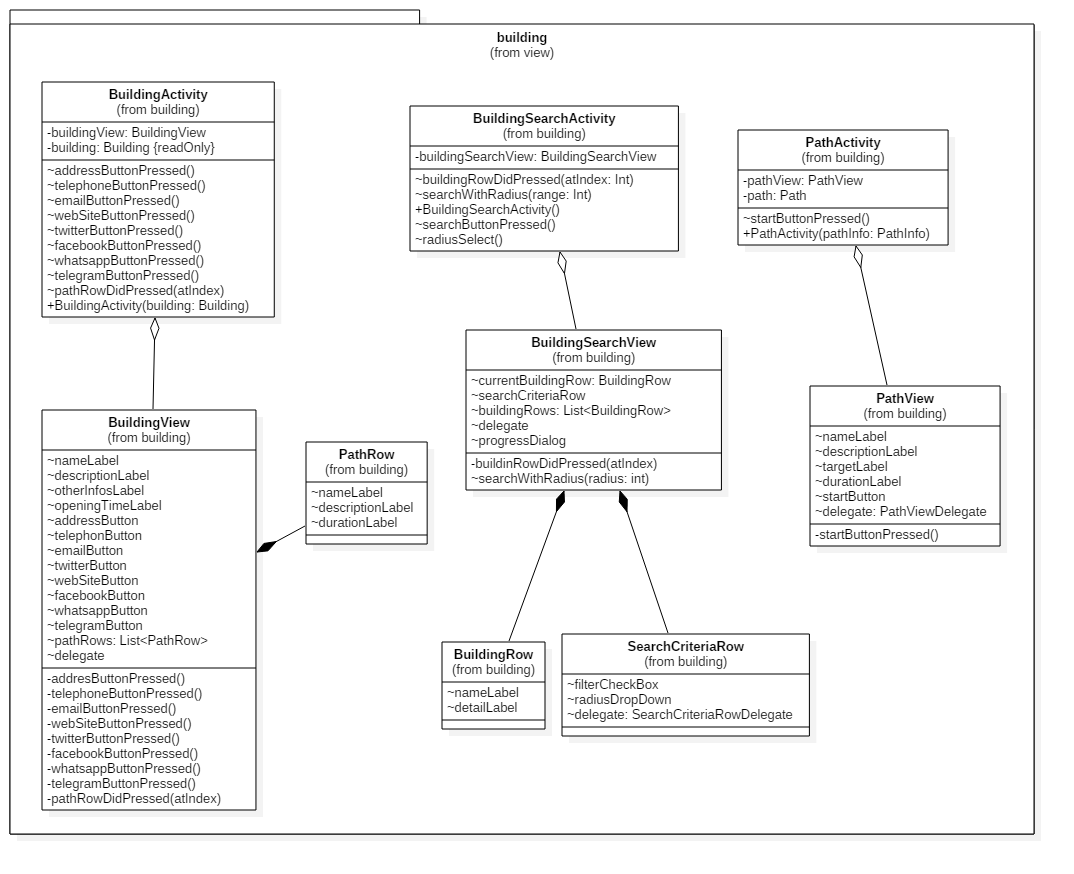
\includegraphics[scale=0.4]{img/package/png/client--viewcontroller--building.png} 
\caption{Schema package client::viewcontroller::building} 
 \end{figure} 
\compDescrizione{componente che gestisce le informazioni e le interazioni dell'utente con gli edifici abilitati}
\compPadre{viewcontroller}
\begin{compClassi} \\ 
\begin{classe}{CLIPS::client::viewcontroller::building::BuildingActivity}
\classeDescrizione{classe controller che si occupa di interagire con BuildingView}
\classeUtilizzo{classe controller che si occupa di interagire con BuildingView}
\begin{classeRelazioni}
\classeRelazione{CLIPS::client::viewcontroller::building}{BuildingView}{classe per la visualizzazione di un edificio}\classeRelazione{CLIPS::client::viewcontroller::building}{BuildingViewDelegate}{interfaccia per segnalare gli eventi della classe BuildingView}\end{classeRelazioni}
\end{classe}\begin{classe}{CLIPS::client::viewcontroller::building::BuildingRow}
\classeDescrizione{classe per la rappresentazione di un edificio nella ricerca}
\classeUtilizzo{permette di visualizzare le informazioni di un edificio nella lista dei risultati di ricerca}
\end{classe}\begin{classe}{CLIPS::client::viewcontroller::building::BuildingSearchActivity}
\classeDescrizione{classe controller che si occupa di interagire con BuildingSearchView}
\classeUtilizzo{si occupa di gestire le interazioni dell'utente con BuildingSearchView}
\begin{classeRelazioni}
\classeRelazione{CLIPS::client::viewcontroller::building}{BuildingSearchView}{classe per la ricerca degli edifici}\classeRelazione{CLIPS::client::viewcontroller::building}{BuildingSearchViewDelegate}{interfaccia per segnalare gli eventi della classe BuildingSearchView}\end{classeRelazioni}
\end{classe}\begin{classe}{CLIPS::client::viewcontroller::building::BuildingSearchView}
\classeDescrizione{classe per la ricerca degli edifici}
\classeUtilizzo{permette all'utente di cercare gli edifici vicini per visualizzare le informazioni e/o i percorsi disponibili}
\begin{classeRelazioni}
\classeRelazione{CLIPS::client::viewcontroller::building}{BuildingRow}{classe per la rappresentazione di un edificio nella ricerca}\classeRelazione{CLIPS::client::viewcontroller::building}{BuildingSearchViewDelegate}{interfaccia per segnalare gli eventi della classe BuildingSearchView}\classeRelazione{CLIPS::client::viewcontroller::building}{SearchCriteriaRow}{classe utilizzata per determinare i criteri di ricerca degli edifici}\end{classeRelazioni}
\end{classe}\begin{classe}{CLIPS::client::viewcontroller::building::BuildingSearchViewDelegate}
\classeDescrizione{interfaccia per segnalare gli eventi della classe BuildingSearchView}
\classeUtilizzo{si occupa di fornire i metodi necessari alla classe BuildingSearchView per notificare gli eventi}
\begin{classeRelazioni}
\classeRelazione{CLIPS::client::viewcontroller::building}{BuildingSearchActivity}{classe controller che si occupa di interagire con BuildingSearchView}\classeRelazione{CLIPS::client::viewcontroller::building}{BuildingSearchView}{classe per la ricerca degli edifici}\end{classeRelazioni}
\end{classe}\begin{classe}{CLIPS::client::viewcontroller::building::BuildingView}
\classeDescrizione{classe per la visualizzazione di un edificio}
\classeUtilizzo{permette all'utente di visualizzare le informazioni relative all'edificio selezionato}
\begin{classeAttributi}
\classeAttributo{addressButton}{void}{rappresenta l'indirizzo dell'edificio}
\classeAttributo{descriptionLabel}{void}{indica la descrizione dell'edificio}
\classeAttributo{emailButton}{void}{indica l'indirizzo email dell'edificio}
\classeAttributo{facebookButton}{void}{indica l'indirizzo facebook dell'edificio}
\classeAttributo{nameLabel}{void}{rappresenta il nome dell'edificio}
\classeAttributo{openingTimeLabel}{void}{rappresenta gli orari di apertura dell'edificio}
\classeAttributo{otherInfosLabel}{void}{rappresenta le altre informazioni sull'edificio}
\classeAttributo{pathRows}{void}{rappresenta la lista dei percorsi dell'edificio}
\classeAttributo{telegramButton}{void}{rappresenta il contatto Telegram dell'edificio}
\classeAttributo{telephoneButton}{void}{rappresenta il numero telefonico dell'edificio}
\classeAttributo{twitterButton}{void}{indica l'indirizzo twitter dell'edificio}
\classeAttributo{webSiteButton}{void}{rappresenta l'indirizzo web dell'edificio}
\classeAttributo{whatsappButton}{void}{indica il contatto WhatsApp dell'edificio}
\end{classeAttributi}
\begin{classeMetodi}
\classeMetodo{addressButtonPressed}{}{void}{notifica al controller l'interazione con addressButton}
\classeMetodo{emailButtonPressed}{}{void}{notifica al controller l'interazione con emailButton}
\classeMetodo{facebookButtonPressed}{}{void}{notifica al controller l'interazione con facebookButton}
\classeMetodo{pathRowDidPressed}{}{void}{notifica al controller l'interazione con pathRow}
\classeMetodo{telegramButtonPressed}{}{void}{notifica al controller l'interazione con telegramButton}
\classeMetodo{telephoneButtonPressed}{}{void}{notifica al controller l'interazione con telephoneButton}
\classeMetodo{twitterButtonPressed}{}{void}{notifica al controller l'interazione con twitterButton}
\classeMetodo{websiteButtonPressed}{}{void}{notifica al controller l'interazione con webSiteButton}
\classeMetodo{whatstappButtonPressed}{}{void}{notifica al controller l'interazione con whatsappButton}
\end{classeMetodi}
\begin{classeRelazioni}
\classeRelazione{CLIPS::client::viewcontroller::building}{BuildingViewDelegate}{interfaccia per segnalare gli eventi della classe BuildingView}\classeRelazione{CLIPS::client::viewcontroller::building}{PathRow}{classe per la rappresentazione di un percorso nella ricerca}\end{classeRelazioni}
\end{classe}\begin{classe}{CLIPS::client::viewcontroller::building::BuildingViewDelegate}
\classeDescrizione{interfaccia per segnalare gli eventi della classe BuildingView}
\classeUtilizzo{si occupa di fornire i metodi necessari alla classe BuildingView per notificare gli eventi}
\end{classe}\begin{classe}{CLIPS::client::viewcontroller::building::PathActivity}
\classeDescrizione{classe controller che si occupa di interagire con PathView}
\classeUtilizzo{si occupa di gestire le interazioni dell'utente con PathView}
\begin{classeRelazioni}
\classeRelazione{CLIPS::client::viewcontroller::building}{PathView}{classe che si occupa della visualizzazione della schermata riguardante un percorso}\classeRelazione{CLIPS::client::viewcontroller::building}{PathViewDelegate}{interfaccia per segnalare gli eventi della classe PathView}\end{classeRelazioni}
\end{classe}\begin{classe}{CLIPS::client::viewcontroller::building::PathRow}
\classeDescrizione{classe per la rappresentazione di un percorso nella ricerca}
\classeUtilizzo{permette un percorso disponibile nella lista dei risultati di ricerca}
\end{classe}\begin{classe}{CLIPS::client::viewcontroller::building::PathView}
\classeDescrizione{classe che si occupa della visualizzazione della schermata riguardante un percorso}
\classeUtilizzo{consente all'utente di visualizzare le informazioni riguardanti un percorso e se l'utente si trova nell'edificio del percorso consente di iniziarlo}
\begin{classeRelazioni}
\classeRelazione{CLIPS::client::viewcontroller::building}{PathViewDelegate}{interfaccia per segnalare gli eventi della classe PathView}\end{classeRelazioni}
\end{classe}\begin{classe}{CLIPS::client::viewcontroller::building::PathViewDelegate}
\classeDescrizione{interfaccia per segnalare gli eventi della classe PathView}
\classeUtilizzo{si occupa di fornire i metodi necessari alla classe PathView per notificare gli eventi}
\begin{classeRelazioni}
\classeRelazione{CLIPS::client::viewcontroller::building}{PathActivity}{classe controller che si occupa di interagire con PathView}\classeRelazione{CLIPS::client::viewcontroller::building}{PathView}{classe che si occupa della visualizzazione della schermata riguardante un percorso}\end{classeRelazioni}
\end{classe}\begin{classe}{CLIPS::client::viewcontroller::building::SearchCriteriaRow}
\classeDescrizione{classe utilizzata per determinare i criteri di ricerca degli edifici}
\classeUtilizzo{permette all'utente di visualizzare i criteri di ricerca disponibili}
\begin{classeRelazioni}
\classeRelazione{CLIPS::client::viewcontroller::building}{SearchCriteriaRowDelegate}{interfaccia per segnalare gli eventi della classe SearchCriteriaRow}\end{classeRelazioni}
\end{classe}\begin{classe}{CLIPS::client::viewcontroller::building::SearchCriteriaRowDelegate}
\classeDescrizione{interfaccia per segnalare gli eventi della classe SearchCriteriaRow}
\classeUtilizzo{si occupa di fornire i metodi necessari alla classe SearchCriteriaRow per notificare gli eventi}
\begin{classeRelazioni}
\classeRelazione{CLIPS::client::viewcontroller::building}{BuildingSearchView}{classe per la ricerca degli edifici}\classeRelazione{CLIPS::client::viewcontroller::building}{SearchCriteriaRow}{classe utilizzata per determinare i criteri di ricerca degli edifici}\end{classeRelazioni}
\end{classe}\end{compClassi}
\end{componente}
\begin{componente}{CLIPS::client::viewcontroller::games}
\begin{figure}[h!] 
\centering 
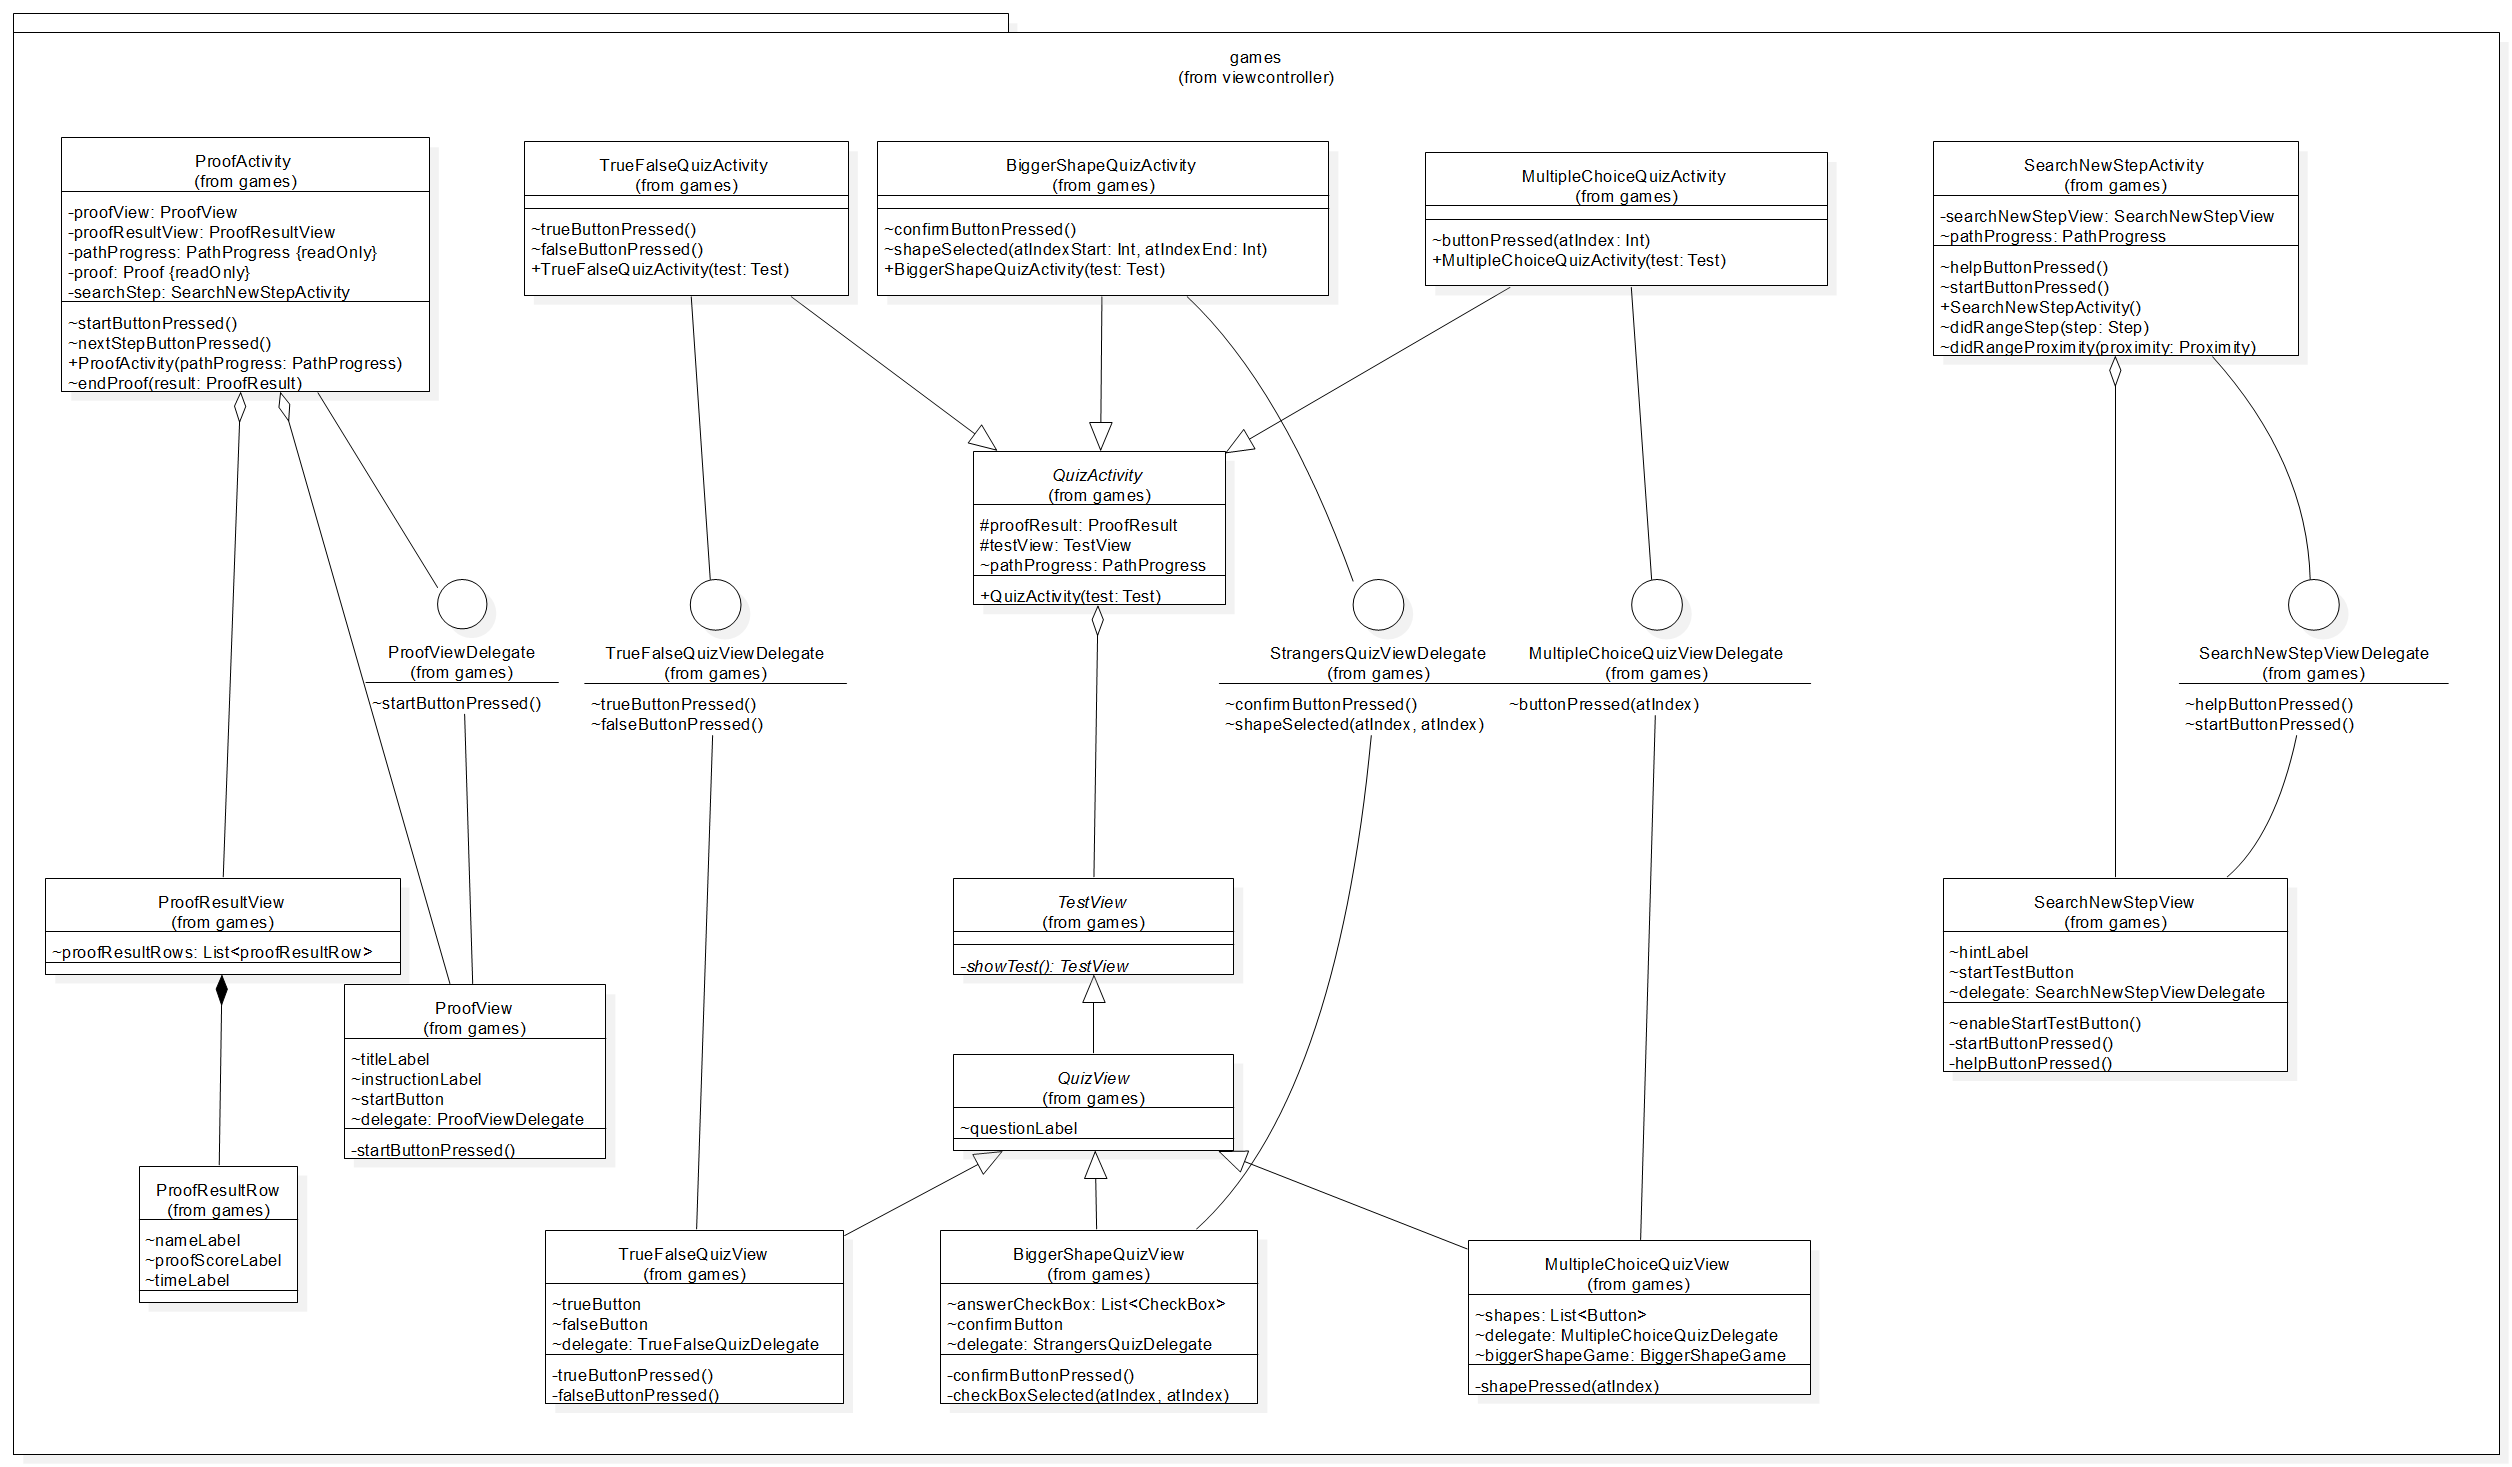
\includegraphics[scale=0.4]{img/package/png/client--viewcontroller--games.png} 
\caption{Schema package client::viewcontroller::games} 
 \end{figure} 
\compDescrizione{componente che gestisce le prove che l'utente deve completare all'interno di un percorso}
\compPadre{viewcontroller}
\begin{compClassi} \\ 
\begin{classe}{CLIPS::client::viewcontroller::games::MultipleChoiceQuizActivity}
\classeDescrizione{classe controller che si occupa di interagire con MultipleChoiceView}
\classeUtilizzo{si occupa di gestire le interazioni dell'utente con MultipleChoiceView}
\begin{classeRelazioni}
\classeRelazione{CLIPS::client::viewcontroller::games}{MultipleChoiceQuizViewDelegate}{interfaccia per segnalare gli eventi della classe MultipleChoiceView}\classeRelazione{CLIPS::client::viewcontroller::games}{QuizActivity}{interfaccia per segnalare gli eventi della classe QuizView}\end{classeRelazioni}
\end{classe}\begin{classe}{CLIPS::client::viewcontroller::games::MultipleChoiceQuizView}
\classeDescrizione{classe per il quiz a risposta multipla}
\classeUtilizzo{si occupa di fornire un'interfaccia per il quiz a risposta multipla}
\begin{classeAttributi}
\classeAttributo{answerButtons}{void}{una lista di buttons per visualizzare le possibili risposte}
\end{classeAttributi}
\begin{classeMetodi}
\classeMetodo{buttonPressed}{atIndex}{void}{segnala al controller il button premuto}
\begin{classeMetodoArgomenti}
\classeMetodoArgomento{atIndex}{int}{indica l'indice della risposta selezionata}
\end{classeMetodoArgomenti}
\end{classeMetodi}
\begin{classeRelazioni}
\classeRelazione{CLIPS::client::viewcontroller::games}{MultipleChoiceQuizViewDelegate}{interfaccia per segnalare gli eventi della classe MultipleChoiceView}\classeRelazione{CLIPS::client::viewcontroller::games}{QuizView}{classe base per i quiz}\end{classeRelazioni}
\end{classe}\begin{classe}{CLIPS::client::viewcontroller::games::MultipleChoiceQuizViewDelegate}
\classeDescrizione{interfaccia per segnalare gli eventi della classe MultipleChoiceView}
\classeUtilizzo{si occupa di fornire i metodi necessari alla classe MultipleChoiceView per notificare gli eventi}
\begin{classeRelazioni}
\classeRelazione{CLIPS::client::viewcontroller::games}{MultipleChoiceQuizActivity}{classe controller che si occupa di interagire con MultipleChoiceView}\classeRelazione{CLIPS::client::viewcontroller::games}{MultipleChoiceQuizView}{classe per il quiz a risposta multipla}\end{classeRelazioni}
\end{classe}\begin{classe}{CLIPS::client::viewcontroller::games::ProofActivity}
\classeDescrizione{classe controller che si occupa di interagire con ProofView}
\classeUtilizzo{si occupa di gestire le interazioni dell'utente con ProofView}
\begin{classeRelazioni}
\classeRelazione{CLIPS::client::viewcontroller::games}{ProofResultView}{classe che rappresenta la schermata dei risultati}\classeRelazione{CLIPS::client::viewcontroller::games}{ProofViewDelegate}{interfaccia per segnalare gli eventi della classe ProofView}\end{classeRelazioni}
\end{classe}\begin{classe}{CLIPS::client::viewcontroller::games::ProofResultRow}
\classeDescrizione{classe che rappresenta una risultato rappresentato all'interno di una riga che può essere cliccata}
\classeUtilizzo{permette all'utente di visualizzare le informazioni generali di un risultato di una prova e di cliccarci per visualizzarne le informazioni dettagliate}
\end{classe}\begin{classe}{CLIPS::client::viewcontroller::games::ProofResultView}
\classeDescrizione{classe che rappresenta la schermata dei risultati}
\classeUtilizzo{permette all'utente di visualizzare le informazioni generali dei risultati delle prove e cliccare sulle prove delle quali vuole visualizzare le informazioni dettagliate}
\begin{classeRelazioni}
\classeRelazione{CLIPS::client::viewcontroller::games}{ProofResultRow}{classe che rappresenta una risultato rappresentato all'interno di una riga che può essere cliccata}\end{classeRelazioni}
\end{classe}\begin{classe}{CLIPS::client::viewcontroller::games::ProofView}
\classeDescrizione{classe che rappresenta la schermata della prova}
\classeUtilizzo{permette all'utente di visualizzare la prova da giocare}
\begin{classeRelazioni}
\classeRelazione{CLIPS::client::viewcontroller::games}{ProofViewDelegate}{interfaccia per segnalare gli eventi della classe ProofView}\end{classeRelazioni}
\end{classe}\begin{classe}{CLIPS::client::viewcontroller::games::ProofViewDelegate}
\classeDescrizione{interfaccia per segnalare gli eventi della classe ProofView}
\classeUtilizzo{si occupa di fornire i metodi necessari alla classe ProofView per notificare gli eventi}
\begin{classeRelazioni}
\classeRelazione{CLIPS::client::viewcontroller::games}{ProofActivity}{classe controller che si occupa di interagire con ProofView}\classeRelazione{CLIPS::client::viewcontroller::games}{ProofView}{classe che rappresenta la schermata della prova}\end{classeRelazioni}
\end{classe}\begin{classe}{CLIPS::client::viewcontroller::games::QuizActivity}
\classeDescrizione{interfaccia per segnalare gli eventi della classe QuizView}
\classeUtilizzo{si occupa di fornire i metodi necessari alla classe QuizView per notificare gli eventi}
\end{classe}\begin{classe}{CLIPS::client::viewcontroller::games::QuizResultView}
\classeDescrizione{classe per la visualizzazione del risultato di un quiz}
\classeUtilizzo{fornisce all'utente un'interfaccia affinché visualizzi il risultato del quiz}
\begin{classeAttributi}
\classeAttributo{continueButton}{void}{button per chiudere la schermata e continuare il percorso}
\classeAttributo{feedbackLabel}{string}{mostra la frase di successo/fallimento del quiz}
\end{classeAttributi}
\begin{classeMetodi}
\classeMetodo{continueButtonPressed}{}{void}{notifica il controller che il button per continuare è stato premuto}
\classeMetodo{showFailureResult}{correctAnswer}{void}{mostra la risposta corretta se il quiz è stato fallito}
\begin{classeMetodoArgomenti}
\classeMetodoArgomento{correctAnswer}{string}{indica la risposta corretta}
\end{classeMetodoArgomenti}
\classeMetodo{showSuccessfulResult}{score}{void}{mostra il risultato ottenuto se il quiz è stato superato}
\begin{classeMetodoArgomenti}
\classeMetodoArgomento{score}{int}{indica il punteggio ottenuto}
\end{classeMetodoArgomenti}
\end{classeMetodi}
\end{classe}\begin{classe}{CLIPS::client::viewcontroller::games::QuizView}
\classeDescrizione{classe base per i quiz}
\classeUtilizzo{fornisce una base per i vari tipi di test da istanziare}
\begin{classeAttributi}
\classeAttributo{questionLabel}{string}{rappresenta la domanda da porre nel quiz}
\end{classeAttributi}
\begin{classeRelazioni}
\classeRelazione{CLIPS::client::viewcontroller::games}{TestView}{classe che fornisce una base dalla quale è possibile creare vari tipi di giochi }\end{classeRelazioni}
\end{classe}\begin{classe}{CLIPS::client::viewcontroller::games::QuizViewDelegate}
\classeDescrizione{interfaccia per segnalare gli eventi della classe QuizView}
\classeUtilizzo{si occupa di fornire i metodi necessari alla classe QuizView per notificare gli eventi}
\end{classe}\begin{classe}{CLIPS::client::viewcontroller::games::SearchNewStepActivity}
\classeDescrizione{classe controller che si occupa di interagire con SearchNewStepView}
\classeUtilizzo{si occupa di gestire le interazioni dell'utente con SearchNewStepView}
\begin{classeRelazioni}
\classeRelazione{CLIPS::client::viewcontroller::games}{SearchNewStepView}{classe che rappresenta la schermata per la ricerca della prossima prova del percorso}\classeRelazione{CLIPS::client::viewcontroller::games}{SearchNewStepViewDelegate}{interfaccia per segnalare gli eventi della classe SearchNewStepView}\end{classeRelazioni}
\end{classe}\begin{classe}{CLIPS::client::viewcontroller::games::SearchNewStepView}
\classeDescrizione{classe che rappresenta la schermata per la ricerca della prossima prova del percorso}
\classeUtilizzo{permette all'utente di cercare in modo semplificato la ricerca della prossima prova del percorso}
\begin{classeRelazioni}
\classeRelazione{CLIPS::client::viewcontroller::games}{SearchNewStepViewDelegate}{interfaccia per segnalare gli eventi della classe SearchNewStepView}\end{classeRelazioni}
\end{classe}\begin{classe}{CLIPS::client::viewcontroller::games::SearchNewStepViewDelegate}
\classeDescrizione{interfaccia per segnalare gli eventi della classe SearchNewStepView}
\classeUtilizzo{si occupa di fornire i metodi necessari alla classe SearchNewStepView per notificare gli eventi}
\begin{classeRelazioni}
\classeRelazione{CLIPS::client::viewcontroller::games}{SearchNewStepActivity}{classe controller che si occupa di interagire con SearchNewStepView}\classeRelazione{CLIPS::client::viewcontroller::games}{SearchNewStepView}{classe che rappresenta la schermata per la ricerca della prossima prova del percorso}\end{classeRelazioni}
\end{classe}\begin{classe}{CLIPS::client::viewcontroller::games::TestResultView}
\classeDescrizione{classe che fornisce una base per la visualizzazione del risultato della prova}
\classeUtilizzo{permette all'utente di visualizzare il risultato della prova}
\begin{classeMetodi}
\classeMetodo{showResult()}{}{void}{restituisce la view con il risultato}
\end{classeMetodi}
\end{classe}\begin{classe}{CLIPS::client::viewcontroller::games::TestView}
\classeDescrizione{classe che fornisce una base dalla quale è possibile creare vari tipi di giochi }
\classeUtilizzo{viene utilizzata per visualizzare un'interfaccia di gioco all'utente}
\begin{classeMetodi}
\classeMetodo{showTest}{}{TestView}{restituisce l'interfaccia grafica del test}
\end{classeMetodi}
\end{classe}\begin{classe}{CLIPS::client::viewcontroller::games::TrueFalseQuizActivity}
\classeDescrizione{classe controller che si occupa di interagire con TrueFalseQuizView}
\classeUtilizzo{si occupa di gestire le interazioni dell'utente con TrueFalseQuizView}
\begin{classeRelazioni}
\classeRelazione{CLIPS::client::viewcontroller::games}{QuizActivity}{interfaccia per segnalare gli eventi della classe QuizView}\classeRelazione{CLIPS::client::viewcontroller::games}{TrueFalseQuizViewDelegate}{interfaccia per segnalare gli eventi della classe TrueFalseQuizView}\end{classeRelazioni}
\end{classe}\begin{classe}{CLIPS::client::viewcontroller::games::TrueFalseQuizView}
\classeDescrizione{classe per il quiz vero/falso}
\classeUtilizzo{si occupa di fornire un'interfaccia per la prova di tipo vero/falso}
\begin{classeAttributi}
\classeAttributo{falseButton}{void}{button grafico per rispondere falso al quiz}
\classeAttributo{trueButton}{void}{button grafico per rispondere vero al quiz}
\end{classeAttributi}
\begin{classeMetodi}
\classeMetodo{falseButtonPressed}{}{void}{questo metodo si occupa di notificare al controller che è stato premuto falseButton}
\classeMetodo{trueButtonPressed}{}{void}{questo metodo si occupa di notificare al controller che è stato premuto trueButton}
\end{classeMetodi}
\begin{classeRelazioni}
\classeRelazione{CLIPS::client::viewcontroller::games}{QuizView}{classe base per i quiz}\classeRelazione{CLIPS::client::viewcontroller::games}{TrueFalseQuizViewDelegate}{interfaccia per segnalare gli eventi della classe TrueFalseQuizView}\end{classeRelazioni}
\end{classe}\begin{classe}{CLIPS::client::viewcontroller::games::TrueFalseQuizViewDelegate}
\classeDescrizione{interfaccia per segnalare gli eventi della classe TrueFalseQuizView}
\classeUtilizzo{si occupa di fornire i metodi necessari alla classe TrueFalseQuizView per notificare gli eventi}
\begin{classeRelazioni}
\classeRelazione{CLIPS::client::viewcontroller::games}{TrueFalseQuizActivity}{classe controller che si occupa di interagire con TrueFalseQuizView}\classeRelazione{CLIPS::client::viewcontroller::games}{TrueFalseQuizView}{classe per il quiz vero/falso}\end{classeRelazioni}
\end{classe}\end{compClassi}
\end{componente}
\begin{componente}{CLIPS::client::viewcontroller::savedresults}
\begin{figure}[h!] 
\centering 
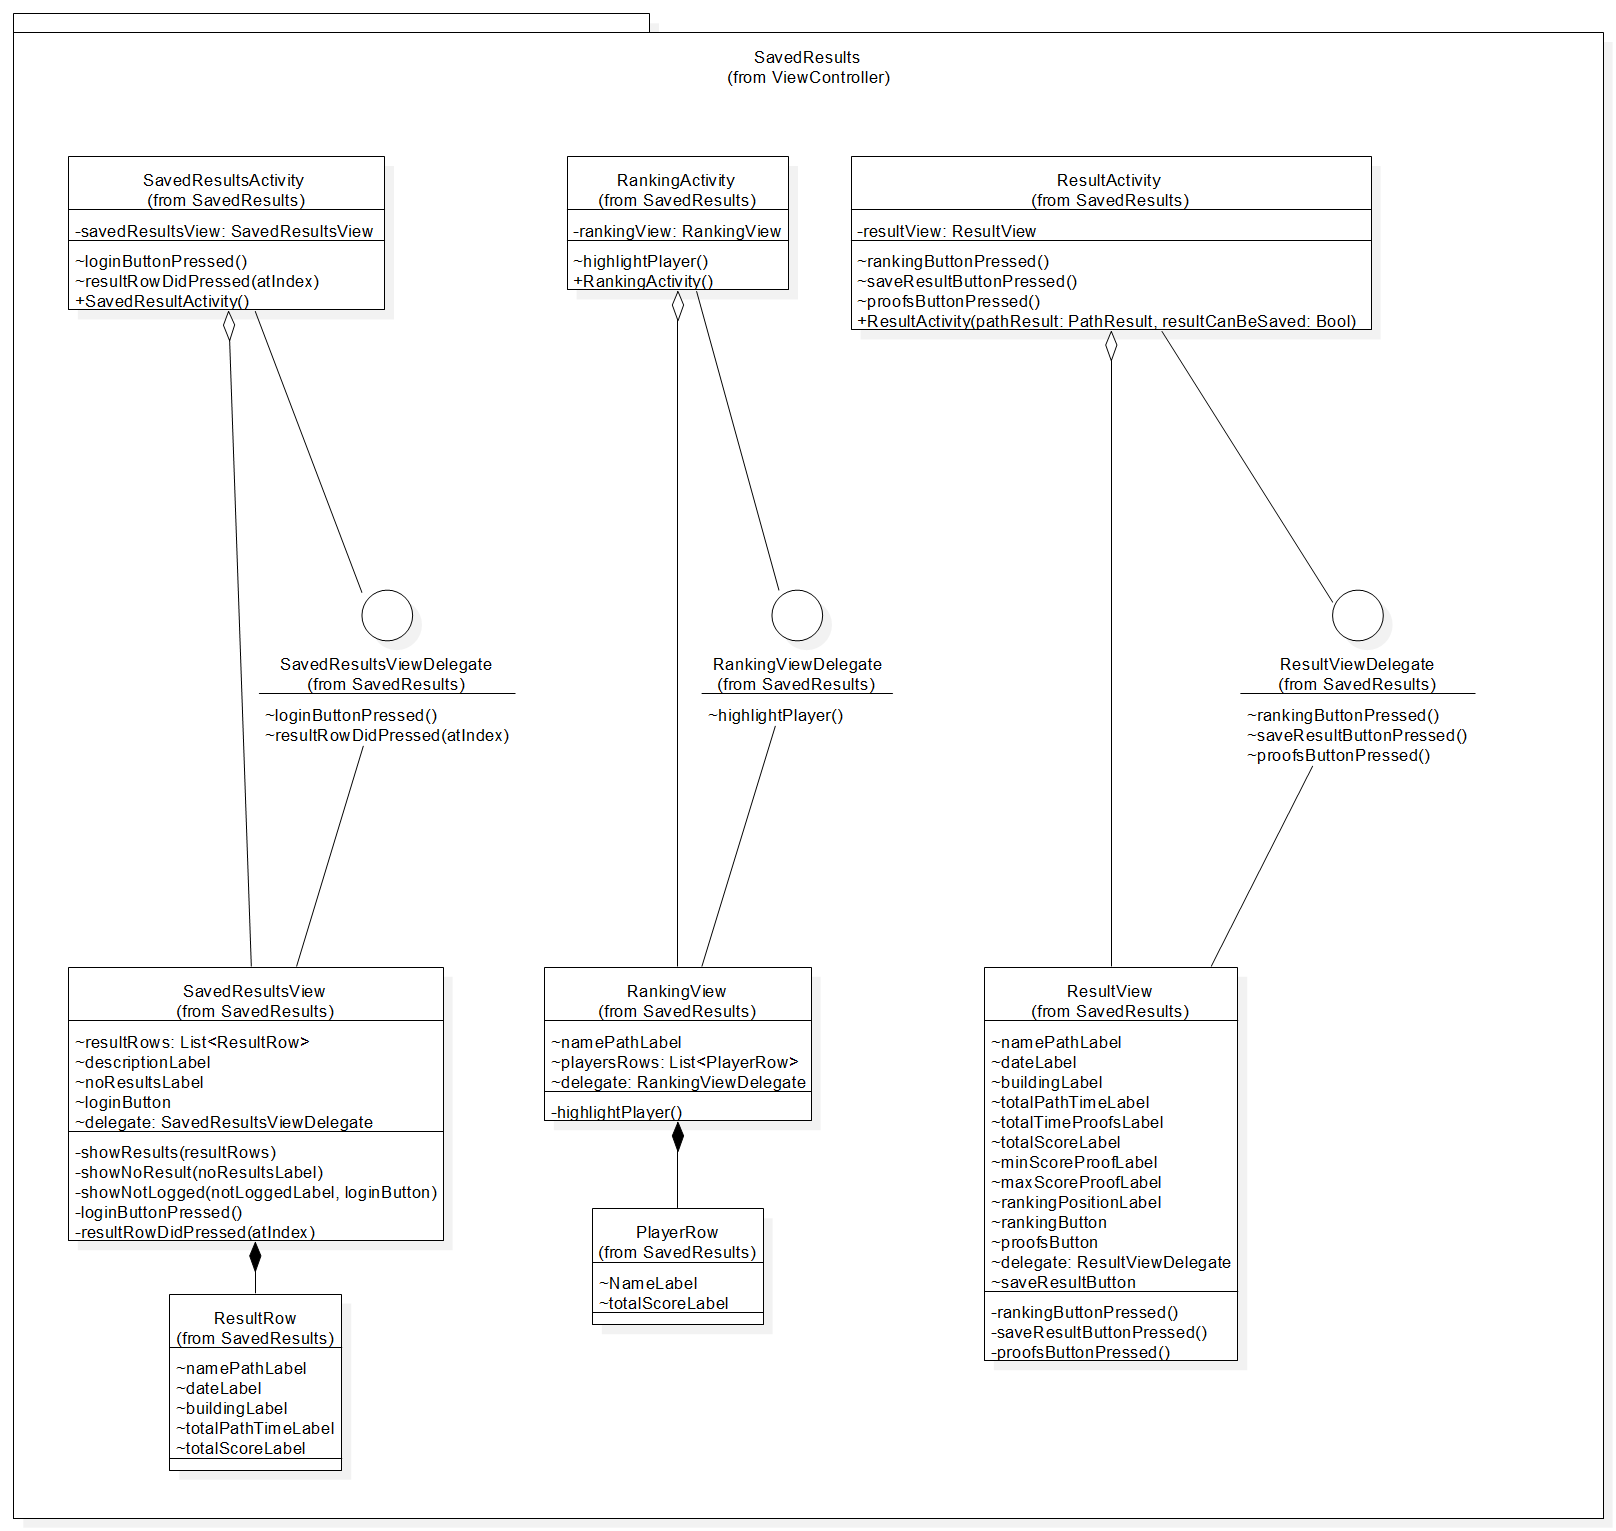
\includegraphics[scale=0.4]{img/package/png/client--viewcontroller--savedresults.png} 
\caption{Schema package client::viewcontroller::savedresults} 
 \end{figure} 
\compDescrizione{componente che raggruppa le le view e i controller dei risultati salvati e delle classifiche}
\compPadre{viewcontroller}
\begin{compClassi} \\ 
\begin{classe}{CLIPS::client::viewcontroller::savedresults::PlayerRow}
\classeDescrizione{classe che rappresenta una riga all'interno di una classifica}
\classeUtilizzo{permette all'utente di visualizzare il nome del giocatore e il suo punteggio nel percorso d'interesse}
\end{classe}\begin{classe}{CLIPS::client::viewcontroller::savedresults::RankingActivity}
\classeDescrizione{classe controller che si occupa di interagire con RankingView}
\classeUtilizzo{si occupa di gestire le interazioni dell'utente con RankingView}
\end{classe}\begin{classe}{CLIPS::client::viewcontroller::savedresults::RankingViewDelegate}
\classeDescrizione{interfaccia per segnalare gli eventi della classe RankingView}
\classeUtilizzo{si occupa di fornire i metodi necessari alla classe RankingView per notificare gli eventi}
\end{classe}\begin{classe}{CLIPS::client::viewcontroller::savedresults::ResultActivity}
\classeDescrizione{classe controller che si occupa di interagire con ResultView}
\classeUtilizzo{si occupa di gestire le interazioni dell'utente con ResultView}
\begin{classeRelazioni}
\classeRelazione{CLIPS::client::viewcontroller::savedresults}{ResultView}{classe che rappresenta la schermata nel quali si possono visualizzare i risultati di un percorso}\classeRelazione{CLIPS::client::viewcontroller::savedresults}{ResultView}{classe che rappresenta la schermata nel quali si possono visualizzare i risultati di un percorso}\classeRelazione{CLIPS::client::viewcontroller::savedresults}{ResultViewDelegate}{interfaccia per segnalare gli eventi della classe ResultView}\end{classeRelazioni}
\end{classe}\begin{classe}{CLIPS::client::viewcontroller::savedresults::ResultRow}
\classeDescrizione{classe che rappresenta una riga di un risultato}
\classeUtilizzo{permette all'utente di visualizzare le informazioni generali di un risultato e di cliccarci per visualizzare quelle dettagliate}
\end{classe}\begin{classe}{CLIPS::client::viewcontroller::savedresults::ResultView}
\classeDescrizione{classe che rappresenta la schermata nel quali si possono visualizzare i risultati di un percorso}
\classeUtilizzo{permette all'utente di visualizzare le informazioni dettagliate del risultato di un percorso}
\begin{classeRelazioni}
\classeRelazione{CLIPS::client::viewcontroller::savedresults}{ResultViewDelegate}{interfaccia per segnalare gli eventi della classe ResultView}\end{classeRelazioni}
\end{classe}\begin{classe}{CLIPS::client::viewcontroller::savedresults::ResultViewDelegate}
\classeDescrizione{interfaccia per segnalare gli eventi della classe ResultView}
\classeUtilizzo{interfaccia per segnalare gli eventi della classe ResultView}
\begin{classeRelazioni}
\classeRelazione{CLIPS::client::viewcontroller::savedresults}{ResultActivity}{classe controller che si occupa di interagire con ResultView}\classeRelazione{CLIPS::client::viewcontroller::savedresults}{ResultView}{classe che rappresenta la schermata nel quali si possono visualizzare i risultati di un percorso}\end{classeRelazioni}
\end{classe}\begin{classe}{CLIPS::client::viewcontroller::savedresults::SavedResultsActivity}
\classeDescrizione{classe controller che si occupa di interagire con SavedResultView}
\classeUtilizzo{si occupa di gestire le interazioni dell'utente con SavedResultView}
\begin{classeRelazioni}
\classeRelazione{CLIPS::client::viewcontroller::savedresults}{SavedResultsViewDelegate}{interfaccia per segnalare gli eventi della classe SavedResultsView}\classeRelazione{CLIPS::client::viewcontroller::savedresults}{SavedResultView}{classe che rappresenta la schermata dei risultati salvati di un utente}\end{classeRelazioni}
\end{classe}\begin{classe}{CLIPS::client::viewcontroller::savedresults::SavedResultsViewDelegate}
\classeDescrizione{interfaccia per segnalare gli eventi della classe SavedResultsView}
\classeUtilizzo{si occupa di fornire i metodi necessari alla classe SavedResultsView per notificare gli eventi}
\begin{classeRelazioni}
\classeRelazione{CLIPS::client::viewcontroller::savedresults}{SavedResultsActivity}{classe controller che si occupa di interagire con SavedResultView}\classeRelazione{CLIPS::client::viewcontroller::savedresults}{SavedResultView}{classe che rappresenta la schermata dei risultati salvati di un utente}\end{classeRelazioni}
\end{classe}\begin{classe}{CLIPS::client::viewcontroller::savedresults::SavedResultView}
\classeDescrizione{classe che rappresenta la schermata dei risultati salvati di un utente}
\classeUtilizzo{permette all'utente di visualizzare i propri risultati salvati}
\begin{classeRelazioni}
\classeRelazione{CLIPS::client::viewcontroller::savedresults}{ResultRow}{classe che rappresenta una riga di un risultato}\classeRelazione{CLIPS::client::viewcontroller::savedresults}{SavedResultsViewDelegate}{interfaccia per segnalare gli eventi della classe SavedResultsView}\end{classeRelazioni}
\end{classe}\end{compClassi}
\end{componente}
\begin{componente}{CLIPS::client::viewcontroller::utility}
\begin{figure}[h!] 
\centering 
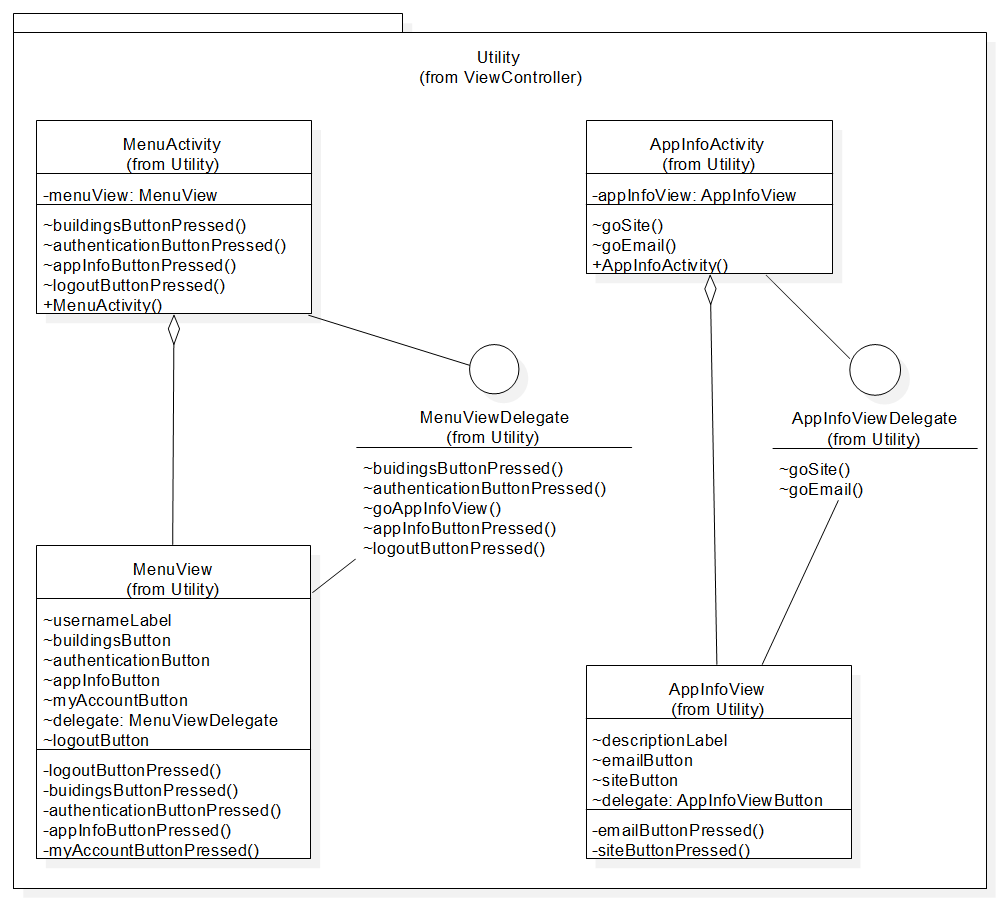
\includegraphics[scale=0.4]{img/package/png/client--viewcontroller--utility.png} 
\caption{Schema package client::viewcontroller::utility} 
 \end{figure} 
\compDescrizione{componente che raggruppa le view generali dell'app}
\compPadre{viewcontroller}
\begin{compClassi} \\ 
\begin{classe}{CLIPS::client::viewcontroller::utility::AppInfoActivity}
\classeDescrizione{classe controller che si occupa di interagire con AppInfoView}
\classeUtilizzo{si occupa di gestire le interazioni dell'utente con AppInfoView}
\begin{classeRelazioni}
\classeRelazione{CLIPS::client::authentication}{AccountViewDelegate}{interfaccia per segnalare gli eventi della classe AccountView}\classeRelazione{CLIPS::client::viewcontroller::utility}{AppInfoView}{classe che si occupa delle informazioni generali dell'app}\end{classeRelazioni}
\end{classe}\begin{classe}{CLIPS::client::viewcontroller::utility::AppInfoView}
\classeDescrizione{classe che si occupa delle informazioni generali dell'app}
\classeUtilizzo{permette all'utente di visualizzare le informazioni generali dell'app}
\begin{classeRelazioni}
\classeRelazione{CLIPS::client::viewcontroller::utility}{AppInfoViewDelegate}{interfaccia per segnalare gli eventi della classe AppInfoView}\end{classeRelazioni}
\end{classe}\begin{classe}{CLIPS::client::viewcontroller::utility::AppInfoViewDelegate}
\classeDescrizione{interfaccia per segnalare gli eventi della classe AppInfoView}
\classeUtilizzo{si occupa di fornire i metodi necessari alla classe AppInfoView per notificare gli eventi}
\begin{classeRelazioni}
\classeRelazione{CLIPS::client::viewcontroller::utility}{AppInfoActivity}{classe controller che si occupa di interagire con AppInfoView}\classeRelazione{CLIPS::client::viewcontroller::utility}{AppInfoView}{classe che si occupa delle informazioni generali dell'app}\end{classeRelazioni}
\end{classe}\begin{classe}{CLIPS::client::viewcontroller::utility::MenuActivity}
\classeDescrizione{classe controller che si occupa di interagire con MenuView}
\classeUtilizzo{si occupa di gestire le interazioni dell'utente con MenuView}
\begin{classeRelazioni}
\classeRelazione{CLIPS::client::viewcontroller::utility}{MenuView}{classe che si occupa di far visualizzare il menu}\classeRelazione{CLIPS::client::viewcontroller::utility}{MenuViewDelegate}{interfaccia per segnalare gli eventi della classe MenuViewDelegate}\end{classeRelazioni}
\end{classe}\begin{classe}{CLIPS::client::viewcontroller::utility::MenuView}
\classeDescrizione{classe che si occupa di far visualizzare il menu}
\classeUtilizzo{consente all'utente di navigare nell'app tramite il menu}
\begin{classeRelazioni}
\classeRelazione{CLIPS::client::viewcontroller::utility}{MenuViewDelegate}{interfaccia per segnalare gli eventi della classe MenuViewDelegate}\end{classeRelazioni}
\end{classe}\begin{classe}{CLIPS::client::viewcontroller::utility::MenuViewDelegate}
\classeDescrizione{interfaccia per segnalare gli eventi della classe MenuViewDelegate}
\classeUtilizzo{si occupa di fornire i metodi necessari alla classe MenuViewDelegate per notificare gli eventi}
\begin{classeRelazioni}
\classeRelazione{CLIPS::client::viewcontroller::utility}{MenuActivity}{classe controller che si occupa di interagire con MenuView}\classeRelazione{CLIPS::client::viewcontroller::utility}{MenuView}{classe che si occupa di far visualizzare il menu}\end{classeRelazioni}
\end{classe}\end{compClassi}
\end{componente}
\begin{componente}{CLIPS::server}
\begin{figure}[h!] 
\centering 
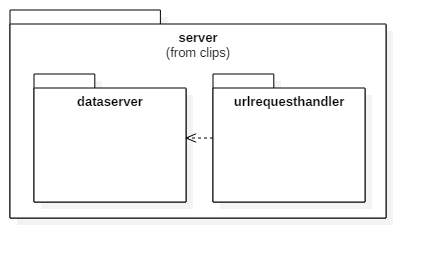
\includegraphics[scale=0.4]{img/package/png/server.png} 
\caption{Schema package server} 
 \end{figure} 
\compDescrizione{componente globale per il back end del prodotto}
\compPadre{CLIPS}
\begin{compPackageContenuti}
\item CLIPS::server::dataserver: package per la gestione dei dati sul server
\item CLIPS::server::urlrequesthandler: componente che gestisce le richieste inviate al server e le risposte da inviare al client
\end{compPackageContenuti}
\end{componente}
\begin{componente}{CLIPS::server::dataserver}
\begin{figure}[h!] 
\centering 
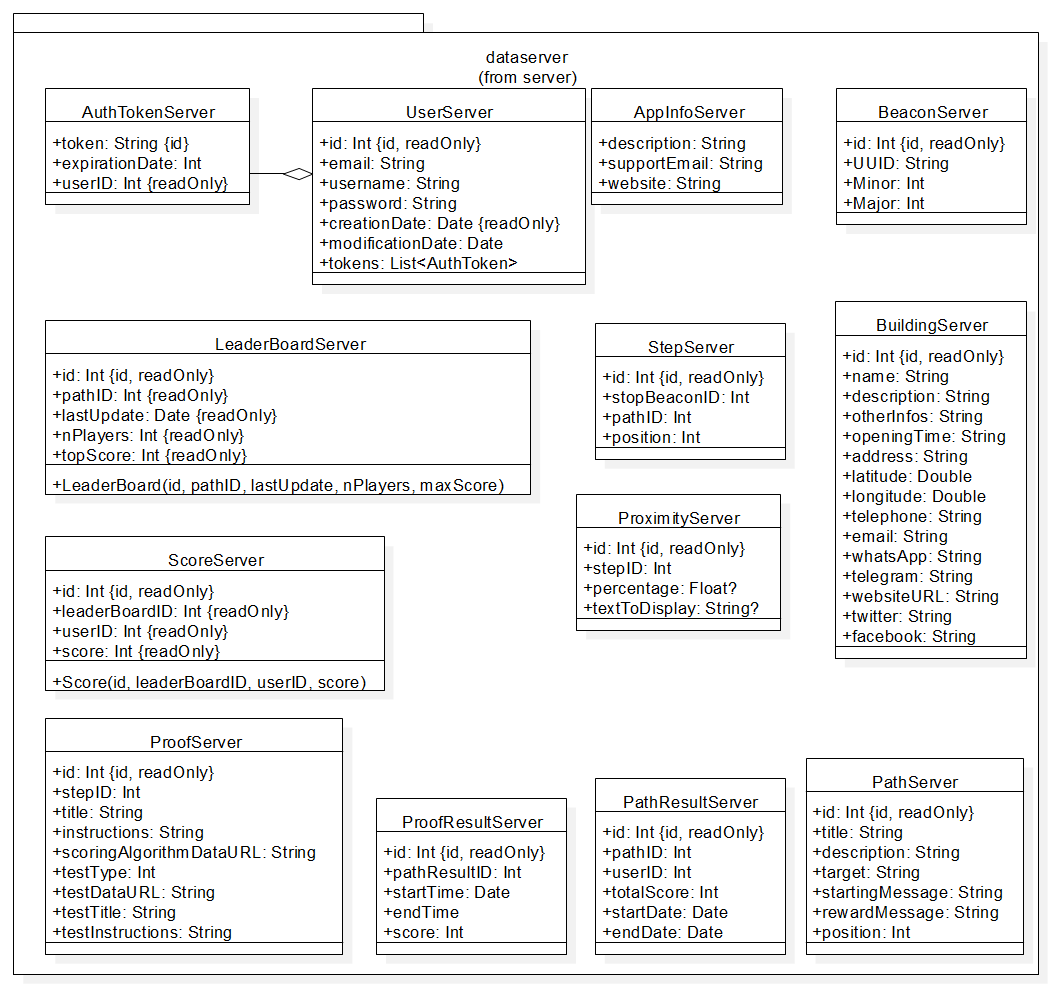
\includegraphics[scale=0.4]{img/package/png/server--data.png} 
\caption{Schema package server::dataserver} 
 \end{figure} 
\compDescrizione{package per la gestione dei dati sul server}
\compPadre{server}
\begin{compClassi} \\ 
\begin{classe}{CLIPS::server::dataserver::AppInfoServer}
\classeDescrizione{classe che rappresenta le informazioni dell'app sul server}
\classeUtilizzo{permette di salvare sul server le informazioni dell'app}
\end{classe}\begin{classe}{CLIPS::server::dataserver::AuthTokenServer}
\classeDescrizione{Classe che rappresenta un token che si riferisce ad un utente loggato}
\classeUtilizzo{permette utilizzare un token per riferirsi ad utente loggato}
\end{classe}\begin{classe}{CLIPS::server::dataserver::BeaconServer}
\classeDescrizione{classe che rappresenta un beacon nel server}
\classeUtilizzo{permette di salvare sul server un beacon}
\end{classe}\begin{classe}{CLIPS::server::dataserver::BuildingServer}
\classeDescrizione{classe che rappresenta un edificio sul server}
\classeUtilizzo{permette di salvare e modificare i dati di un edificio sul server}
\end{classe}\begin{classe}{CLIPS::server::dataserver::LeaderBoardServer}
\classeDescrizione{classe che rappresenta la classifica sul server}
\classeUtilizzo{permette di salvare i dati della classifica sul server}
\end{classe}\begin{classe}{CLIPS::server::dataserver::PathResultServer}
\classeDescrizione{classe che rappresenta il risultato di un percorso sul server}
\classeUtilizzo{consente di salvare i risultati di un percorso sul server}
\end{classe}\begin{classe}{CLIPS::server::dataserver::PathServer}
\classeDescrizione{classe che rappresenta un percorso sul server}
\classeUtilizzo{permette di creare, modificare ed eliminare un percorso sul server}
\end{classe}\begin{classe}{CLIPS::server::dataserver::ProofResultServer}
\classeDescrizione{classe che rappresenta i risultati di una prova sul server}
\classeUtilizzo{consente di salvare il risultato di una prova sul server}
\end{classe}\begin{classe}{CLIPS::server::dataserver::ProofServer}
\classeDescrizione{classe che rappresenta una prova sul server}
\classeUtilizzo{permette di creare, modificare ed eliminare una prova sul server}
\end{classe}\begin{classe}{CLIPS::server::dataserver::ProximityServer}
\classeDescrizione{classe che rappresenta sul server un beacon indicato alla segnalazione della distanza dalla prossima prova}
\classeUtilizzo{permette di salvare i beacon di segnalazione sul server}
\end{classe}\begin{classe}{CLIPS::server::dataserver::ScoreManager}
\classeDescrizione{classe che rappresenta un risultato sul server}
\classeUtilizzo{permette si salvare un risultato nel server}
\end{classe}\begin{classe}{CLIPS::server::dataserver::StepServer}
\classeDescrizione{classe che rappresenta uno step di un percorso nel server}
\classeUtilizzo{permette di salvare sul server uno step di un percorso}
\end{classe}\begin{classe}{CLIPS::server::dataserver::UserServer}
\classeDescrizione{classe che rappresenta un utente nel server}
\classeUtilizzo{permette di salvare sul server un utente}
\begin{classeRelazioni}
\classeRelazione{CLIPS::server::dataserver}{AuthTokenServer}{Classe che rappresenta un token che si riferisce ad un utente loggato}\end{classeRelazioni}
\end{classe}\end{compClassi}
\end{componente}
\begin{componente}{CLIPS::server::urlrequesthandler}
\begin{figure}[h!] 
\centering 
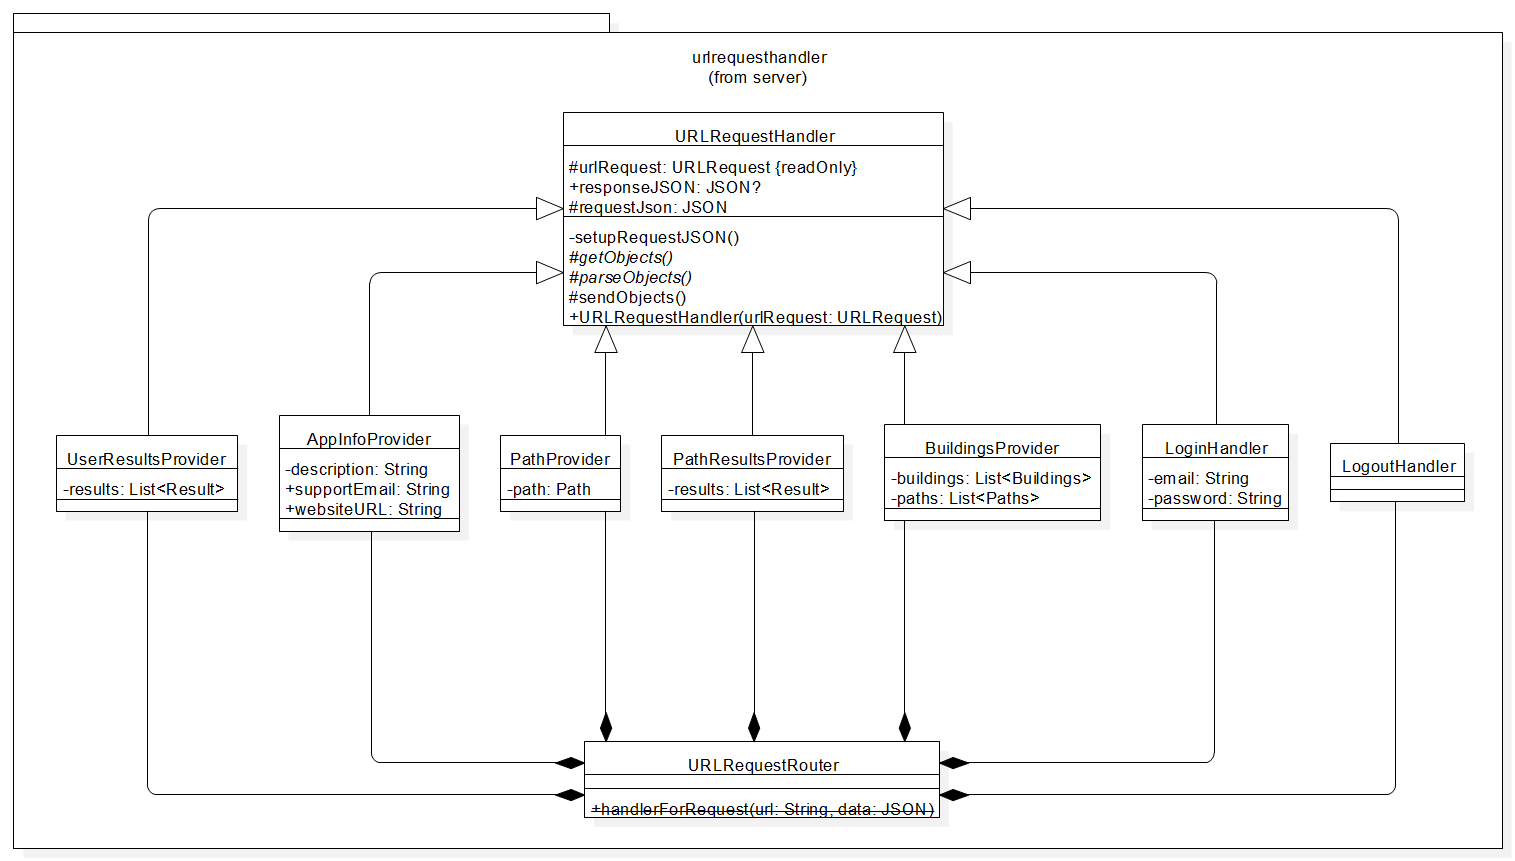
\includegraphics[scale=0.4]{img/package/png/server--urlrequesthandler.png} 
\caption{Schema package server::urlrequesthandler} 
 \end{figure} 
\compDescrizione{componente che gestisce le richieste inviate al server e le risposte da inviare al client}
\compPadre{server}
\begin{compClassi} \\ 
\begin{classe}{CLIPS::server::urlrequesthandler::AppInfoProvider}
\classeDescrizione{classe che gestisce la richiesta di informazioni dell'app}
\classeUtilizzo{si occupa di restituire le informazioni dell'app richieste}
\end{classe}\begin{classe}{CLIPS::server::urlrequesthandler::BuildingsProvider}
\classeDescrizione{classe che gestisce la richiesta degli edifici dal client}
\classeUtilizzo{si occupa di restituire le informazioni sugli edifici richieste}
\end{classe}\begin{classe}{CLIPS::server::urlrequesthandler::LoginHandler}
\classeDescrizione{classe che rappresenta le informazioni per il login}
\classeUtilizzo{si occupa di gestire il login lato server}
\end{classe}\begin{classe}{CLIPS::server::urlrequesthandler::LogoutHandler}
\classeDescrizione{classe che rappresenta il logout}
\classeUtilizzo{si occupa di effettuare il logout}
\end{classe}\begin{classe}{CLIPS::server::urlrequesthandler::PathProvider}
\classeDescrizione{classe che gestisce la richiesta del percorso dal client}
\classeUtilizzo{si occupa di restituire le informazioni sul percorso richieste}
\end{classe}\begin{classe}{CLIPS::server::urlrequesthandler::PathResultsProvider}
\classeDescrizione{classe che gestisce la richiesta del risultato del percorso dal client}
\classeUtilizzo{si occupa di restituire le informazioni del risultato sul percorso richieste}
\end{classe}\begin{classe}{CLIPS::server::urlrequesthandler::URLRequestHandler}
\classeDescrizione{classe che rappresenta il gestore delle richieste nel server}
\classeUtilizzo{si occupa di gestire le richieste ricevute dal client}
\end{classe}\begin{classe}{CLIPS::server::urlrequesthandler::URLRequestRouter}
\classeDescrizione{classe che si occupa di creare il corretto URLRequestHandler per gestire la richiesta HTTP rivolta al server}
\classeUtilizzo{crea la classe URLRequestHandler appropriata}
\begin{classeRelazioni}
\classeRelazione{CLIPS::server::urlrequesthandler}{AppInfoProvider}{classe che gestisce la richiesta di informazioni dell'app}\classeRelazione{CLIPS::server::urlrequesthandler}{AppInfoProvider}{classe che gestisce la richiesta di informazioni dell'app}\classeRelazione{CLIPS::server::urlrequesthandler}{BuildingsProvider}{classe che gestisce la richiesta degli edifici dal client}\classeRelazione{CLIPS::server::urlrequesthandler}{LoginHandler}{classe che rappresenta le informazioni per il login}\classeRelazione{CLIPS::server::urlrequesthandler}{LogoutHandler}{classe che rappresenta il logout}\classeRelazione{CLIPS::server::urlrequesthandler}{PathProvider}{classe che gestisce la richiesta del percorso dal client}\classeRelazione{CLIPS::server::urlrequesthandler}{PathResultsProvider}{classe che gestisce la richiesta del risultato del percorso dal client}\classeRelazione{CLIPS::server::urlrequesthandler}{UserResultProvider}{classe che gestisce la richiesta di un utente}\end{classeRelazioni}
\end{classe}\begin{classe}{CLIPS::server::urlrequesthandler::UserResultProvider}
\classeDescrizione{classe che gestisce la richiesta di un utente}
\classeUtilizzo{si occupa di restituire gli utenti richiesti dal client}
\end{classe}\end{compClassi}
\end{componente}
